%%%%%%%%%%%%%%%%%%%%%%%%%%%%%%%%%%%%%%%%%%%%%%%%%%%%%%%%%%%%%%%%%%%%%%%%%%%%%%%%
%% 
%%%%%%%%%%%%%%%%%%%%%%%%%%%%%%%%%%%%%%%%%%%%%%%%%%%%%%%%%%%%%%%%%%%%%%%%%%%%%%%%

\documentclass[a4paper, 12pt]{book}

%%-- Geometría principal (dejar activada la siguiente línea en la versión final)
\usepackage[a4paper, left=2.5cm, right=2.5cm, top=3cm, bottom=3cm]{geometry}
%%-- Activar esta línea y comentar la anterior en modo borrador, para comentarios al margen
%\usepackage[a4paper, left=2.5cm, right=2.5cm, top=3cm, bottom=3cm, marginparwidth=60pt]{geometry}

%%-- Hay que cargarlo antes que las traducciones
\usepackage{listing}                    % Listados de código

% Traducciones en XeLaTeX
% \usepackage{polyglossia}
%\setmainlanguage{spanish}    % Comenta esta línea si tu memoria es en inglés

% Traducciones particulares para español
% Caption tablas
%\gappto\captionsspanish{
%	\def\tablename{Tabla}
%	\def\listingscaption{Código}
%	\def\refname{Bibliografía}
%	\def\appendixname{Apéndice}
%	\def\listtablename{Índice de tablas}
%	\def\listingname{Código}
% 	\def\listlistingname{Índice de fragmentos de código}
%}

%% Tipografía y estilos
\usepackage[OT1]{fontenc}               % Keeps eulervm happy about accents encoding

% Símbolos y fuentes matemáticas elegantes: Euler virtual math fonts
% ¡Importante! Carga siempre las fuentes math AMS Euler ANTES QUE fontspec
\usepackage{amsmath}
\usepackage{amssymb}
\usepackage[OT1,euler-digits,euler-hat-accent,small]{eulervm}

% En XeLaTeX las fuentes se especifican con fontspec
\usepackage{fontspec}
\defaultfontfeatures{Scale=MatchLowercase, Ligatures=TeX}     % Default option in font config

% Fix para fuentes usadas con operadores y \mathrm
\DeclareSymbolFont{operators}{\encodingdefault}{\familydefault}{m}{n}

% Configura la fuente principal (serif): MinionPro
\setmainfont[Scale=0.96]{TeX Gyre Pagella}
% Configura la fuente sans-serif (\sffamily)
\setsansfont[Scale=MatchLowercase]{Lato}
% Configura la fuente para letra monoespaciada: Source Code Pro, escala 0.85
\setmonofont[Scale=0.85]{Source Code Pro}

%%-- Familias de fuentes específicas
%%-- Se pueden definir etiquetas para familias de fuentes personalizadas
%%-- que luego puedes emplear para cambiar el formato de una parte de texto
%%-- Ejemplo:
% \newfontfamily{\myriadprocond}{Myriad Pro Semibold Condensed.otf}

%%-- Opciones de interlineado y espacios
\linespread{1.07}                   % Aumentar interlineado para fuentes tipo Palatino
\setlength{\parskip}{\baselineskip} % Separar párrafos con línea en blanco

%%-- Hipervínculos
\usepackage{url}

%%-- Gráficos y tablas
\PassOptionsToPackage{dvipdfmx,usenames,dvipsnames,x11names,table}{xcolor}             % Definiciones de colores
\PassOptionsToPackage{xetex}{graphicx}

\usepackage{subfig}                     % Subfiguras
\usepackage{pgf}
\usepackage{svg}                        % Integración de imágenes en formato SVG
\usepackage{float}                      % H para posicionar figuras
\usepackage{booktabs}                   % Already loads package xcolor
\usepackage{multicol}                   % multiple column layout facilities
\usepackage{colortbl}                   % For coloured tables

%%-- Bibliografía con Biblatex y Biber
% Más info:
% https://www.overleaf.com/learn/latex/Biblatex_bibliography_styles
% https://www.overleaf.com/learn/latex/biblatex_citation_styles
\usepackage[british]{babel}
\usepackage[
    style=numeric,
    sorting=none
    ]{biblatex}
\addbibresource{memoria.bib}
% \DeclareFieldFormat{url}{\mkbibacro{URL}\addcolon\nobreakspace\url{#1}}
%\usepackage[nottoc, notlot, notlof, notindex]{tocbibind} %% Opciones de índice

%%-- Matemáticas e ingeniería
% El paquete units permite mostrar unidades correctamente
% Permite escribir unidades con espaciado y estilo de fuente correctos
\usepackage{units}         
% Ejemplo de uso: $\unit[100]{m}$ or $\unitfrac[100]{m}{s}$
% Entornos matemáticos
\newtheorem{theorem}{Theorem}

% Paquetes adicionales
\usepackage{url}                        %% Gestión correcta de enlaces
\usepackage{float}                      %% H para posicionar figuras
\usepackage[nottoc, notlot, notlof, notindex]{tocbibind}    %% Opciones de índice
\usepackage{metalogo}                   %% Múltiples logos para XeLaTeX

% Fuentes especiales y glifos
\usepackage{ccicons}                % Creative Commons icons
\usepackage{metalogo}               % XeTeX logo
\usepackage{fontawesome5}           % Fontawesome 5 icons
\usepackage{adforn} 

% Blindtext
% Opciones pangram, bible, random (defecto)
\usepackage[pangram]{blindtext}
% Lorem ipsum
\usepackage{lipsum}
% Kant lipsum
\usepackage{kantlipsum}

\usepackage{fancyvrb}               % Entornos verbatim extendidos
	\fvset{fontsize=\normalsize}    % Tamaño de fuente por defecto en fancy-verbatim
	
% Configura listas (itemize, enumerate) con iconos personalizados
% Fácil reinicio de numeración con enumerate
% Info: http://ctan.org/pkg/enumitem
\usepackage[shortlabels]{enumitem}
% Usar \usageitem para configurar iconos personalizados en listas
\newcommand{\usageitem}[1]{%
	\item[%
	{\makebox[2em]{\strut\color{GSyCblue} #1}}%
	]
}

%%-- Definición de colores personalizados
% \definecolor{LightGrey}{HTML}{EEEEEE}
% \definecolor{darkred}{rgb}{0.5,0,0}     %% Refs. cruzadas
% \definecolor{darkgreen}{rgb}{0,0.5,0}   %% Citas bibliográficas
% \definecolor{darkblue}{rgb}{0,0,0.5}    %% Hiperenlaces ordinarios (también ToC)

%%-- Configuración fragmentos de código
%%-- Minted necesita Python Pygments instalado en el sistema para funcionar
%%-- En Overleaf ya está instalada esta dependencia
\usepackage[labelfont=bf]{caption}
\newcommand{\source}[1]{\vspace{-3pt} \caption*{Source: {#1}} }
\usepackage{minted}
\usemintedstyle{vs}

%%-- Se debe cargar aquí para evitar warnings
\usepackage{csquotes}                   % Para traducciones con biblatex

%%-- Glosario de términos
% \usepackage[acronym]{glossaries}
% \makeglossaries
% \loadglsentries{glossary}

% % Definición de cabeceras del documento, usando fancyhdr
% \usepackage{fancyhdr}
% %% Configuración de cabeceras para el cuerpo principal del documento
% \pagestyle{fancy}
% \fancyhead{}
% \fancyhead[RO,LE]{\myriadprocond{\thepage}}
% \renewcommand{\chaptermark}[1]{\markboth{\chaptername\ \thechapter.\ #1}{}}
% \renewcommand{\sectionmark}[1]{\markright{\thesection.\ #1}}
% \fancyhead[RE]{\myriadprocond{\leftmark}}
% \fancyhead[LO]{\myriadprocond{\rightmark}}
% \renewcommand{\headrulewidth}{0pt}
% \setlength{\headheight}{15pt} %% Al menos 15pt para evitar warning al compilar
% \fancyfoot{}
% %% Configuración para páginas con cabecera en blanco
% \fancypagestyle{plain}{%
% \fancyhf{}% clear all header and footer fields
% \fancyhead[RO,LE]{\myriadprocond{\thepage}}
% \renewcommand{\headrulewidth}{0pt}%
% \renewcommand{\footrulewidth}{0pt}%
% }

%%%%%%%%%%%%%%%%%%%
%% Own changes
%%%%%%%%%%%%%%%%%%%
\newenvironment{conditions}[1][where:]
  {#1 \begin{tabular}[t]{>{$}l<{$} @{${}={}$} l}}
  {\end{tabular}\\[\belowdisplayskip]}
\raggedbottom


%%%%%%%%%%%%%%%%%%%%%%%%%%%%%%%%%%%%%%%%

%%-- Metadatos del doc
\title{Memoria del Proyecto}
\author{Nombre del autor}

%%-- Hiperenlaces, siempre se carga al final del preámbulo
\usepackage[colorlinks]{hyperref}
\hypersetup{
    pdftoolbar=true,	% Muestra barra de herramientas en Adobe Acrobat
	pdfmenubar=true,	% Muestra menú en Adobe Acrobat
	pdftitle={Título doc en ventana del visor o navegador},
	pdfauthor={Nombre del alumno/a},
	pdfcreator={ETSII/ETSIT, URJC},
	pdfproducer={XeLaTeX},
	pdfsubject={Topic1, Topic2, Topic3},
	pdfnewwindow=true,              %links open in new window
    colorlinks=true,                % false: boxed links; true: coloured links
    linkcolor=Firebrick4,           % enlaces internos 
    citecolor=Aquamarine4,          % enlaces a citas bibliográficas
    urlcolor=RoyalBlue3,            % hiperenlances ordinarios
    linktocpage=true                % Enlaces en núm. pág. en ToC
}

%%%---------------------------------------------------------------------------
% Comentarios en línea de revisión
% Este bloque se puede borrar cuando finalizamos el borrador

\usepackage[colorinlistoftodos]{todonotes}
\usepackage{verbatim}
%%%---------------------------------------------------------------------------

\begin{document}

%%-- Configuración común para todos los entornos listing
%%-- Descomentar para usar y personalizar valores
%\lstset{%
%breakatwhitespace=true,
% breaklines=true, 
% basicstyle=\footnotesize\ttfamily,
% keywordstyle=\color{blue},
% commentstyle=\color{green!40!black}, 
% language=Python} 
 

%%%%%%%%%%%%%%%%%%%%%%%%%%%%%%%%%%%%%%%%%%%%%%%%%%%%%%%%%%%%%%%%%%%%%%%%%%%%%%%%
% PORTADA

\begin{titlepage}
\begin{center}
\begin{tabular}[c]{c c}
%\includegraphics[bb=0 0 194 352, scale=0.25]{logo} &
\includegraphics[scale=1.5]{img/LogoURJC.png}
%&
%\begin{tabular}[b]{l}
%\Huge
%\textsf{UNIVERSIDAD} \\
%\Huge
%\textsf{REY JUAN CARLOS} \\
%\end{tabular}
\\
\end{tabular}

\vspace{3cm}

\Large 
GRADO EN INGENIERÍA AEROESPACIAL EN AERONAVEGACIÓN

\vspace{0.4cm}

\large
Curso Académico 2022/2023

\vspace{0.8cm}

Trabajo Fin de Grado

\vspace{2cm}

\LARGE Exploration of vision-based \\
control solutions for PX4-driven UAVs
\vspace{3cm}

\large
Autora : Laura González Fernández \\
Tutores : Xin Chen, Alejandro Sáez Mollejo
\end{center}
\end{titlepage}

\newpage
\mbox{}
\thispagestyle{empty} % para que no se numere esta pagina


%%%%%%%%%%%%%%%%%%%%%%%%%%%%%%%%%%%%%%%%%%%%%%%%%%%%%%%%%%%%%%%%%%%%%%%%%%%%%%%%
%%%% Para firmar
\clearpage
\pagenumbering{gobble}
\chapter*{}

\vspace{-4cm}
\begin{center}
\LARGE
\textbf{Trabajo Fin de Grado}

\vspace{1cm}
\large
Exploration of Vision-Based Control Solutions for PX4-Driven UAVs.

\vspace{1cm}
\large
\textbf{Autora :} Laura González Fernández \\
\textbf{Tutores :} Xin Chen, Alejandro Sáez Mollejo

\end{center}

\vspace{1cm}
La defensa del presente Proyecto Fin de Grado/Máster se realizó el día 3\qquad$\;\,$ de
\qquad\qquad\qquad\qquad \newline de 20XX, siendo calificada por el siguiente tribunal:


\vspace{0.5cm}
\textbf{Presidente:}

\vspace{0.8cm}
\textbf{Secretario:}

\vspace{0.8cm}
\textbf{Vocal:}


\vspace{0.8cm}
y habiendo obtenido la siguiente calificación:

\vspace{0.8cm}
\textbf{Calificación:}


\vspace{0.8cm}
\begin{flushright}
Móstoles/Fuenlabrada, a \qquad$\;\,$ de \qquad\qquad\qquad\qquad de 20XX
\end{flushright}

%%%%%%%%%%%%%%%%%%%%%%%%%%%%%%%%%%%%%%%%%%%%%%%%%%%%%%%%%%%%%%%%%%%%%%%%%%%%%%%%
%%%% Dedicatoria

\chapter*{}
%\pagenumbering{Roman} % para comenzar la numeración de paginas en numeros romanos
\begin{flushright}
\textit{Aquí normalmente \\
se inserta una dedicatoria corta \\}
\end{flushright}

%%%%%%%%%%%%%%%%%%%%%%%%%%%%%%%%%%%%%%%%%%%%%%%%%%%%%%%%%%%%%%%%%%%%%%%%%%%%%%%%
%%%% Agradecimientos

\chapter*{Agradecimientos}
%\addcontentsline{toc}{chapter}{Agradecimientos} % si queremos que aparezca en el índice
\markboth{AGRADECIMIENTOS}{AGRADECIMIENTOS} % encabezado 

Aquí vienen los agradecimientos\ldots

Hay más espacio para explayarse y explicar a quién agradeces su apoyo o ayuda para
haber acabado el proyecto: familia, pareja, amigos, compañeros de clase\ldots

También hay quien, en algunos casos, hasta agradecer a su tutor o tutores del proyecto
la ayuda prestada\ldots

%%%%%%%%%%%%%%%%%%%%%%%%%%%%%%%%%%%%%%%%%%%%%%%%%%%%%%%%%%%%%%%%%%%%%%%%%%%%%%%%
%%%% Resumen

\chapter*{Resumen}
%\addcontentsline{toc}{chapter}{Resumen} % si queremos que aparezca en el índice
\markboth{RESUMEN}{RESUMEN} % encabezado

Aquí viene un resumen del proyecto.
Ha de constar de tres o cuatro párrafos, donde se presente de manera clara y concisa de qué va el proyecto. 
Han de quedar respondidas las siguientes preguntas:

\begin{itemize}
  \item ¿De qué va este proyecto? ¿Cuál es su objetivo principal?
  \item ¿Cómo se ha realizado? ¿Qué tecnologías están involucradas?
  \item ¿En qué contexto se ha realizado el proyecto? ¿Es un proyecto dentro de un marco general?
\end{itemize}

Lo mejor es escribir el resumen al final.

%%%%%%%%%%%%%%%%%%%%%%%%%%%%%%%%%%%%%%%%%%%%%%%%%%%%%%%%%%%%%%%%%%%%%%%%%%%%%%%%
%%%% Resumen en inglés

\chapter*{Abstract}
%\addcontentsline{toc}{chapter}{Summary} % si queremos que aparezca en el índice
\markboth{ABSTRACT}{ABSTRACT} % encabezado

The popular open-source platform PX4 aims to facilitate the programming of unmanned aerial vehicles and their integration with new sensors and actuators and make it approachable for the common developer. This thesis aims to demonstrate how this platform can be used to develop solutions that integrate computer vision techniques and use their input to control the movement of an aerial vehicle, while employing easily-available and affordable hardware with basic specifications. For this purpose, a viable solution is presented that allows a drone to use an onboard camera to identify and keep track of a person in its field of view to follow their movement.

%%%%--------------------------------------------------------------------
% Lista de comentarios de revisión
% Se puede borrar este bloque al acabar el borrador

\listoftodos
\markboth{TODO LIST}{TODO LIST} % encabezado
%%%%--------------------------------------------------------------------

%%%%%%%%%%%%%%%%%%%%%%%%%%%%%%%%%%%%%%%%%%%%%%%%%%%%%%%%%%%%%%%%%%%%%%%%%%%%%%%%
%%%%%%%%%%%%%%%%%%%%%%%%%%%%%%%%%%%%%%%%%%%%%%%%%%%%%%%%%%%%%%%%%%%%%%%%%%%%%%%%
% ÍNDICES %
%%%%%%%%%%%%%%%%%%%%%%%%%%%%%%%%%%%%%%%%%%%%%%%%%%%%%%%%%%%%%%%%%%%%%%%%%%%%%%%%

% Las buenas noticias es que los índices se generan automáticamente.
% Lo único que tienes que hacer es elegir cuáles quieren que se generen,
% y comentar/descomentar esa instrucción de LaTeX.

%%-- Índice de contenidos
\tableofcontents 
\cleardoublepage
%%-- Índice de figuras
\addcontentsline{toc}{chapter}{List of figures} % para que aparezca en el indice de contenidos
\listoffigures % indice de figuras
\cleardoublepage
%%-- Índice de tablas
%\addcontentsline{toc}{chapter}{Lista de tablas} % para que aparezca en el indice de contenidos
%\listoftables % indice de tablas
% \cleardoublepage
%%-- Índice de fragmentos de código
\addcontentsline{toc}{chapter}{List of listings} % para que aparezca en el indice de contenidos
\listoflistings

%%%%%%%%%%%%%%%%%%%%%%%%%%%%%%%%%%%%%%%%%%%%%%%%%%%%%%%%%%%%%%%%%%%%%%%%%%%%%%%%
%%%%%%%%%%%%%%%%%%%%%%%%%%%%%%%%%%%%%%%%%%%%%%%%%%%%%%%%%%%%%%%%%%%%%%%%%%%%%%%%
%%%%%%%%%%%%%%%%%%%%%%%%%%%%%%%%%%%%%%%%%%%%%%%%%%%%%%%%%%%%%%%%%%%%%%%%%%%%%%%%
%%%%%%%%%%%%%%%%%%%%%%%%%%%%%%%   CONTENT   %%%%%%%%%%%%%%%%%%%%%%%%%%%%%%%%%%%%
%%%%%%%%%%%%%%%%%%%%%%%%%%%%%%%%%%%%%%%%%%%%%%%%%%%%%%%%%%%%%%%%%%%%%%%%%%%%%%%%
%%%%%%%%%%%%%%%%%%%%%%%%%%%%%%%%%%%%%%%%%%%%%%%%%%%%%%%%%%%%%%%%%%%%%%%%%%%%%%%%
%%%%%%%%%%%%%%%%%%%%%%%%%%%%%%%%%%%%%%%%%%%%%%%%%%%%%%%%%%%%%%%%%%%%%%%%%%%%%%%%

% INTRODUCTION %
\cleardoublepage
\chapter{Introduction}
\label{sec:intro}
\pagenumbering{arabic} % para empezar la numeración de página con números

\section{The Dronecontrol project}



%%-- Objetivos del  proyecto
%%-- Si la sección anterior ha quedado muy extensa, se puede considerar convertir
%%-- Las siguientes tres secciones en un capítulo independiente de la memoria

\section{Objectives}
\label{sec:objetives}
\todo[inline]{Write: objectives}

%%%%%%%%%%%%%%%%%%%%%%%%%%%%%
% •	Main Objectives:  
% o	detect + track + follow with vision control techiniques
% o	explore software and hardware possibilities for vision control
% o	machine learning techniques for vision control
% o	SIL/HIL validation procedure
%%%%%%%%%%%%%%%%%%%%%%%%%%%%%


% \subsection{General goal} % título de subsección (se muestra)
% \label{sec:objetivo-general} % identificador de subsección (no se muestra, es para poder referenciarla)
% Aquí vendría el objetivo general en una frase:
% Mi Trabajo Fin de Grado/Master consiste en crear de una herramienta de análisis de los comentarios jocosos en repositorios de software libre alojados en la plataforma GitHub.
% Recuerda que los objetivos siempre vienen en infinitivo.
% \subsection{Specific goals}
% \label{sec:objetivos-especificos}
% Los objetivos específicos se pueden entender como las tareas en las que se ha desglosado el objetivo general. Y, sí, también vienen en infinitivo.
% Lo mejor suele ser utilizar una lista no numerada, como sigue:
%     \begin{itemize}
%         \item Un objetivo específico.
%         \item Otro objetivo específico.
%         \item Tercer objetivo específico.
%         \item \ldots
%     \end{itemize}

\section{Time planning}
\label{sec:time-planning}
\todo[inline]{Polish: time planning}

% Es conveniente que incluyas una descripción de lo que te ha llevado realizar el trabajo.
% Hay gente que añade un diagrama de GANTT.
% Lo importante es que quede claro cuánto tiempo has consumido en realizar el TFG/TFM 
% (tiempo natural, p.ej., 6 meses) y a qué nivel de esfuerzo (p.ej., principalmente los 
% fines de semana).

\section{Thesis layout}
\label{sec:layout}
\todo[inline]{Write: layout}

% Por último, en esta sección se introduce a alto nivel la organización del resto del documento
% y qué contenidos se van a encontrar en cada capítulo.
%     \begin{itemize}
%       \item En el primer capítulo se hace una breve introducción al proyecto, se describen los objetivos del mismo y se refleja la planificación temporal.
%       \item En el siguiente capítulo se describen las tecnologías utilizadas en el desarrollo de este TFM/TFG (Capítulo~\ref{chap:tecnologias}).
%       \item En el capítulo~\ref{chap:desing} Se describe el proceso de desarrollo
%       de la herramienta \ldots
%       \item En el capítulo~\ref{chap:experimentos} Se presentan las principales pruebas realizadas
%       para validación de la plataforma/herramienta\ldots (o resultados de los experimentos
%       efectuados).
%       \item Por último, se presentan las conclusiones del proyecto así como los trabajos futuros que podrían derivarse de éste (Capítulo~\ref{chap:conclusiones}).
%     \end{itemize}

\cleardoublepage
\chapter{State of the art}
\label{chap:sota}
\section{Literature review}
\begin{enumerate}

\item Ref~\cite{Mao2017345} Indoor Follow Me Drone
Tracking through acoustic signals in indoor environments produced by speakers on the drone and received by a mobile device. Discards CV for stability and processing power. Controller on mobile device with three degrees of freedom, pitch and yaw through MPC and roll through PID, with prediction of target's movement.
\begin{itemize}
\item Identification and path following control of an AR.Drone quadrotor \href{https://www.scopus.com/record/display.uri?eid=2-s2.0-84893212045&origin=reflist}{--Link--} \\ 
Path following application based on IMC position controllers, external webcam video stream.

\item Tracking a ground moving target with a quadrotor using switching control: Nonlinear modeling and control \href{https://www.scopus.com/record/display.uri?eid=2-s2.0-84871633622&origin=reflist}{--Link--} \\ 
Tracking of a moving target on ground, embedded camera, use of 2-dimensional images to compute the relative 3-dimensional position and translational velocity of the UAV with respect to the target, switching controllers.

\item A computer vision and control algorithm to follow a human target in a generic environment using a drone \href{https://www.scopus.com/record/display.uri?eid=2-s2.0-84978870802&origin=reflist}{--Link--} \\ 
Tracking and following a generic human target, using the HOG classifier, and on local brightness information, using the optical flow algorithm.

\item Framework for autonomous on-board navigation with the AR.Drone \href{https://www.scopus.com/record/display.uri?eid=2-s2.0-84899426060&origin=reflist}{--Link--} \\ 
All sensing and computations on-board, three systems to autonomously following several trajectory patterns, visually estimate its position and detecting and following a person.

\item A robust real-time embedded vision system on an unmanned rotorcraft for ground target following \href{https://www.scopus.com/record/display.uri?eid=2-s2.0-80054803865&origin=reflist}{--Link--} \\

\item UAV path following for constant line-of-sight \href{https://www.scopus.com/record/display.uri?eid=2-s2.0-85088181184&origin=reflist}{--Link--} \\ 
Flight path guidance and synchronous camera angles to observe a target, analytic expressions are derived for trajectories required for constant line-of-sight orientation relative to the aircraft.

\item Reactive control of autonomous drones \href{https://www.scopus.com/record/display.uri?eid=2-s2.0-84979920485&origin=reflist}{--Link--} \\ 
Reactive control that supersedes the time-triggered approach, control decisions are taken only upon recognizing the need to, based on observed changes in the navigation sensors, rate of execution dynamically adapts to the circumstances.

\item Correlation filter based visual trackers for person pursuit using a low-cost Quadrotor \href{https://www.scopus.com/record/display.uri?eid=2-s2.0-84954554999&origin=reflist}{--Link--} \\ 
Correlation filters for short-term tracking and a redetection strategy based on tracking-learning-detection (TLD), flight experiments in unconstrained environments using human targets and an existing visual servoing controller.

\item The Navigation and Control technology inside the AR.Drone micro UAV \href{https://www.scopus.com/record/display.uri?eid=2-s2.0-84863704626&origin=reflist}{--Link--} \\ 
Navigation and Control technology embedded in a recently commercialized micro Unmanned Aerial Vehicle (UAV), the AR.Drone.

\item Vector field path following for miniature air vehicles \href{https://www.scopus.com/record/display.uri?eid=2-s2.0-34447327237&origin=reflist}{--Link--} \\ 
Method for accurate path following for miniature air vehicles is developed, vector-field path-following control laws are developed for straight-line paths and circular arcs and orbits.

\item Trajectory tracking for autonomous vehicles: An integrated approach to guidance and control \href{https://www.scopus.com/record/display.uri?eid=2-s2.0-0031673631&origin=reflist}{--Link--} \\

\item Trajectory-tracking and path-following of underactuated autonomous vehicles with parametric modeling uncertainty \href{https://www.scopus.com/record/display.uri?eid=2-s2.0-34548237452&origin=reflist}{--Link--} \\

\item Combined trajectory tracking and path following: An application to the coordinated control of autonomous marine craft \href{https://www.scopus.com/record/display.uri?eid=2-s2.0-0035713115&origin=reflist}{--Link--} \\ 
Good trajectory tracking performance while keeping some of the desired properties normally associated with path following

\item Understanding the basis of the kalman filter via a simple and intuitive derivation [lecture notes] \href{https://www.scopus.com/record/display.uri?eid=2-s2.0-85032780920&origin=reflist}{--Link--} \\
\end{itemize}

\item Ref~\cite{Pestana20141886} Computer Vision Based General Object Following for GPS-denied Multirotor Unmanned Vehicles, Ref~\cite{Pestana2013} (6) Vision based GPS-denied Object Tracking and Following for Unmanned Aerial Vehicles
Object tracker + IBVS controllers

\item Ref~\cite{Chakrabarty201625} Autonomous Indoor Object Tracking with the Parrot AR.Drone
Deformable Object
Tracking (CMT) tracker with image-based visual servoing (IBVS), relies directly on image features to compute control values as opposed to position-based servoing

\item Ref~\cite{Bartak201635} Any Object Tracking and Following by a Flying Drone
 Offboard control solution though WiFi on Parrot AR Drone with computer vision (Training-Learning-Detection), with two PID controllers for forward/backward (scale estimation) and yaw (center position).

\end{enumerate}
\newpage
\section{Technologies employed}

\subsection{Software libraries}

\subsubsection{PX4 autopilot}
\label{subsec:px4}
PX4 \footnote{\url{https://docs.px4.io/main/en/}} is a professional open-source autopilot flight stack developed in C++ by developers from industry and academia, and supported by an active world-wide community,
it powers all kinds of vehicles from racing and cargo drones through to ground vehicles and submersibles.
The flight stack software runs on a vehicle controller or flight controller hardware. It supports both Ready To Fly vehicles and custom builds made from scratch,
as well as many additional kinds of sensors and peripherals, such as distance and obstacle sensors, GPS, camera payloads and onboard computers.

PX4 is a core part of a broader drone platform, the Dronecode Project \footnote{\url{https://www.dronecode.org/}}, that includes the QGroundControl ground station \todo{cite}, Pixhawk hardware,
and MAVSDK for integration with companion computers, cameras and other hardware using the MAVLink protocol.
PX4 was initially designed to run on Pixhawk Series controllers, but can now run on Linux computers and other hardware.
The software controls the vehicles through flight modes. 
Flight modes define how the autopilot responds to remote control input, and how it manages vehicle movement during fully autonomous flight.
The modes provide different types or levels of autopilot assistance to the user, ranging from automation of common tasks like takeoff and landing, 
to mechanisms that make it easier to regain level flight or hold the vehicle to a fixed path or position.

\subsubsection{MAVLink and MavSDK}
\label{subsec:mavlink}
MAVLink \footnote{\url{https://mavlink.io/en/}} is a very lightweight messaging protocol for communicating with drones and between onboard drone components. 
It follows a modern hybrid publish-subscribe and point-to-point design pattern 
where data streams are published as topics while configuration sub-protocols 
such as the mission protocol or parameter protocol are sent as point-to-point with retransmission. 
Messages are defined within XML files. 
Each XML file defines the message set supported by a particular MAVLink system.

MAVSDK \footnote{\url{https://mavsdk.mavlink.io/main/en/index.html}} is a collection of libraries for various programming languages,
to interface with MAVLink systems such as drones, cameras or ground systems.
It is primarly written in C++ with wrappers available for,
among others, Swift, Python and Java.
The libraries provides a simple API for managing one or more vehicles, 
providing programmatic access to vehicle information and telemetry, 
and control over missions, movement and other operations.
The libraries can be used onboard a drone on a companion computer
or on the ground for a ground station or mobile device.
MAVSDK is cross-platform: Linux, macOS, Windows, Android and iOS.


\subsubsection{AirSim}
\label{subsec:airsim}
AirSim \footnote{\url{https://microsoft.github.io/AirSim/}} is a simulator for drones, cars and more, built on Unreal Engine and developed by Microsoft. It is open-source, cross platform, and supports software-in-the-loop \gls{sitl} simulation with popular flight controllers such as PX4 and ArduPilot and hardware-in-loop \gls{hitl} with PX4 for physically and visually realistic simulations. It is developed as an Unreal plugin that can simply be dropped into any Unreal environment.

Its goal is to develop a platform for AI research to experiment with deep learning, computer vision and reinforcement learning algorithms for autonomous vehicles. For this purpose, AirSim also exposes APIs to retrieve data and control vehicles in a platform independent way.

\subsubsection{MediaPipe}
\label{subsec:mediapipe}
Mediapipe \footnote{\url{https://google.github.io/mediapipe/}} is an open-source project developed by Google that offers cross-platform, customizable machine learning solutions for live and streaming media.
It supports End-to-End acceleration with built-in fast ML inference and processing accelerated even on common hardware and a unified solution that works across Android, iOS, desktop/cloud, web and IoT.
It offers a framework designed specifically for complex perception pipelines, like real-time perception of human pose, face landmarks and hand tracking that can enable a variety of impactful applications, such as fitness and sport analysis, gesture control and sign language recognition, augmented reality effects and more. 


\subsection{Hardware employed}
\subsubsection{Holybro X500 + Pixhawk 4}
\label{subsec:pixhawk}
The Holybro X500 \footnote{\url{https://docs.px4.io/main/en/frames_multicopter/holybro_x500_pixhawk4.html}} kit is composed of a full carbon-fiber twill frame and the Pixhawk 4 flight controller, 
an advanced autopilot designed and made in collaboration with Holybro and the PX4 team.
It is based on the Pixhawk-project \footnote{\url{https://pixhawk.org/}} FMUv5 open hardware design and it is optimized to run PX4 on the NuttX OS \footnote{\url{https://nuttx.apache.org/}}.
The Pixhawk 4 has an integrated accelerometer/gyroscope, a magnetomer and a barometer.
The kit also includes a power management board, motors an GPS module, an RC receiver and a telemetry radio.
\todo[inline]{More about this in validation (complete build)}


\subsubsection{Raspberry Pi 4}
\label{subsec:rpi}
The Raspberry Pi \footnote{\url{https://www.raspberrypi.com/products/raspberry-pi-4-model-b/}} is a line of single-board computers that stands out thanks to its affordable price,
compact size and maker-friendly design. The model 4B is an improved version of its predecessors,
getting a major increase in processing power, enhanced video output and peripheral connectivity,
while maintaining the same low price and tiny size offered on past models.
This small computer comes as a bare circuit board,
without any sort of housing or add-ons such as a cooling fan or a power button,
but it includes USB, HDMI and Ethernet ports and both Wi-Fi and Bluetooth connectivity,
as well as a 40-pin GPIO \gls{gpio} header, a row of input/output pins that provides direct access for connecting external devices.
The Raspberry Pi runs natively Raspbian OS, a free operating system based on Debian optimized for the Pi hardware, but it is compatible with other standard flavours of Linux.

\subsubsection{Real Sense T265}
\url{https://www.intelrealsense.com/tracking-camera-t265/}

\cleardoublepage

% ESTADO DEL ARTE %
\chapter{State of the art}
\label{chap:sota}
\section{Literature review}
\begin{enumerate}

\item Ref~\cite{Mao2017345} Indoor Follow Me Drone
Tracking through acoustic signals in indoor environments produced by speakers on the drone and received by a mobile device. Discards CV for stability and processing power. Controller on mobile device with three degrees of freedom, pitch and yaw through MPC and roll through PID, with prediction of target's movement.
\begin{itemize}
\item Identification and path following control of an AR.Drone quadrotor \href{https://www.scopus.com/record/display.uri?eid=2-s2.0-84893212045&origin=reflist}{--Link--} \\ 
Path following application based on IMC position controllers, external webcam video stream.

\item Tracking a ground moving target with a quadrotor using switching control: Nonlinear modeling and control \href{https://www.scopus.com/record/display.uri?eid=2-s2.0-84871633622&origin=reflist}{--Link--} \\ 
Tracking of a moving target on ground, embedded camera, use of 2-dimensional images to compute the relative 3-dimensional position and translational velocity of the UAV with respect to the target, switching controllers.

\item A computer vision and control algorithm to follow a human target in a generic environment using a drone \href{https://www.scopus.com/record/display.uri?eid=2-s2.0-84978870802&origin=reflist}{--Link--} \\ 
Tracking and following a generic human target, using the HOG classifier, and on local brightness information, using the optical flow algorithm.

\item Framework for autonomous on-board navigation with the AR.Drone \href{https://www.scopus.com/record/display.uri?eid=2-s2.0-84899426060&origin=reflist}{--Link--} \\ 
All sensing and computations on-board, three systems to autonomously following several trajectory patterns, visually estimate its position and detecting and following a person.

\item A robust real-time embedded vision system on an unmanned rotorcraft for ground target following \href{https://www.scopus.com/record/display.uri?eid=2-s2.0-80054803865&origin=reflist}{--Link--} \\

\item UAV path following for constant line-of-sight \href{https://www.scopus.com/record/display.uri?eid=2-s2.0-85088181184&origin=reflist}{--Link--} \\ 
Flight path guidance and synchronous camera angles to observe a target, analytic expressions are derived for trajectories required for constant line-of-sight orientation relative to the aircraft.

\item Reactive control of autonomous drones \href{https://www.scopus.com/record/display.uri?eid=2-s2.0-84979920485&origin=reflist}{--Link--} \\ 
Reactive control that supersedes the time-triggered approach, control decisions are taken only upon recognizing the need to, based on observed changes in the navigation sensors, rate of execution dynamically adapts to the circumstances.

\item Correlation filter based visual trackers for person pursuit using a low-cost Quadrotor \href{https://www.scopus.com/record/display.uri?eid=2-s2.0-84954554999&origin=reflist}{--Link--} \\ 
Correlation filters for short-term tracking and a redetection strategy based on tracking-learning-detection (TLD), flight experiments in unconstrained environments using human targets and an existing visual servoing controller.

\item The Navigation and Control technology inside the AR.Drone micro UAV \href{https://www.scopus.com/record/display.uri?eid=2-s2.0-84863704626&origin=reflist}{--Link--} \\ 
Navigation and Control technology embedded in a recently commercialized micro Unmanned Aerial Vehicle (UAV), the AR.Drone.

\item Vector field path following for miniature air vehicles \href{https://www.scopus.com/record/display.uri?eid=2-s2.0-34447327237&origin=reflist}{--Link--} \\ 
Method for accurate path following for miniature air vehicles is developed, vector-field path-following control laws are developed for straight-line paths and circular arcs and orbits.

\item Trajectory tracking for autonomous vehicles: An integrated approach to guidance and control \href{https://www.scopus.com/record/display.uri?eid=2-s2.0-0031673631&origin=reflist}{--Link--} \\

\item Trajectory-tracking and path-following of underactuated autonomous vehicles with parametric modeling uncertainty \href{https://www.scopus.com/record/display.uri?eid=2-s2.0-34548237452&origin=reflist}{--Link--} \\

\item Combined trajectory tracking and path following: An application to the coordinated control of autonomous marine craft \href{https://www.scopus.com/record/display.uri?eid=2-s2.0-0035713115&origin=reflist}{--Link--} \\ 
Good trajectory tracking performance while keeping some of the desired properties normally associated with path following

\item Understanding the basis of the kalman filter via a simple and intuitive derivation [lecture notes] \href{https://www.scopus.com/record/display.uri?eid=2-s2.0-85032780920&origin=reflist}{--Link--} \\
\end{itemize}

\item Ref~\cite{Pestana20141886} Computer Vision Based General Object Following for GPS-denied Multirotor Unmanned Vehicles, Ref~\cite{Pestana2013} (6) Vision based GPS-denied Object Tracking and Following for Unmanned Aerial Vehicles
Object tracker + IBVS controllers

\item Ref~\cite{Chakrabarty201625} Autonomous Indoor Object Tracking with the Parrot AR.Drone
Deformable Object
Tracking (CMT) tracker with image-based visual servoing (IBVS), relies directly on image features to compute control values as opposed to position-based servoing

\item Ref~\cite{Bartak201635} Any Object Tracking and Following by a Flying Drone
 Offboard control solution though WiFi on Parrot AR Drone with computer vision (Training-Learning-Detection), with two PID controllers for forward/backward (scale estimation) and yaw (center position).

\end{enumerate}
\newpage
\section{Technologies employed}

\subsection{Software libraries}

\subsubsection{PX4 autopilot}
\label{subsec:px4}
PX4 \footnote{\url{https://docs.px4.io/main/en/}} is a professional open-source autopilot flight stack developed in C++ by developers from industry and academia, and supported by an active world-wide community,
it powers all kinds of vehicles from racing and cargo drones through to ground vehicles and submersibles.
The flight stack software runs on a vehicle controller or flight controller hardware. It supports both Ready To Fly vehicles and custom builds made from scratch,
as well as many additional kinds of sensors and peripherals, such as distance and obstacle sensors, GPS, camera payloads and onboard computers.

PX4 is a core part of a broader drone platform, the Dronecode Project \footnote{\url{https://www.dronecode.org/}}, that includes the QGroundControl ground station \todo{cite}, Pixhawk hardware,
and MAVSDK for integration with companion computers, cameras and other hardware using the MAVLink protocol.
PX4 was initially designed to run on Pixhawk Series controllers, but can now run on Linux computers and other hardware.
The software controls the vehicles through flight modes. 
Flight modes define how the autopilot responds to remote control input, and how it manages vehicle movement during fully autonomous flight.
The modes provide different types or levels of autopilot assistance to the user, ranging from automation of common tasks like takeoff and landing, 
to mechanisms that make it easier to regain level flight or hold the vehicle to a fixed path or position.

\subsubsection{MAVLink and MavSDK}
\label{subsec:mavlink}
MAVLink \footnote{\url{https://mavlink.io/en/}} is a very lightweight messaging protocol for communicating with drones and between onboard drone components. 
It follows a modern hybrid publish-subscribe and point-to-point design pattern 
where data streams are published as topics while configuration sub-protocols 
such as the mission protocol or parameter protocol are sent as point-to-point with retransmission. 
Messages are defined within XML files. 
Each XML file defines the message set supported by a particular MAVLink system.

MAVSDK \footnote{\url{https://mavsdk.mavlink.io/main/en/index.html}} is a collection of libraries for various programming languages,
to interface with MAVLink systems such as drones, cameras or ground systems.
It is primarly written in C++ with wrappers available for,
among others, Swift, Python and Java.
The libraries provides a simple API for managing one or more vehicles, 
providing programmatic access to vehicle information and telemetry, 
and control over missions, movement and other operations.
The libraries can be used onboard a drone on a companion computer
or on the ground for a ground station or mobile device.
MAVSDK is cross-platform: Linux, macOS, Windows, Android and iOS.


\subsubsection{AirSim}
\label{subsec:airsim}
AirSim \footnote{\url{https://microsoft.github.io/AirSim/}} is a simulator for drones, cars and more, built on Unreal Engine and developed by Microsoft. It is open-source, cross platform, and supports software-in-the-loop \gls{sitl} simulation with popular flight controllers such as PX4 and ArduPilot and hardware-in-loop \gls{hitl} with PX4 for physically and visually realistic simulations. It is developed as an Unreal plugin that can simply be dropped into any Unreal environment.

Its goal is to develop a platform for AI research to experiment with deep learning, computer vision and reinforcement learning algorithms for autonomous vehicles. For this purpose, AirSim also exposes APIs to retrieve data and control vehicles in a platform independent way.

\subsubsection{MediaPipe}
\label{subsec:mediapipe}
Mediapipe \footnote{\url{https://google.github.io/mediapipe/}} is an open-source project developed by Google that offers cross-platform, customizable machine learning solutions for live and streaming media.
It supports End-to-End acceleration with built-in fast ML inference and processing accelerated even on common hardware and a unified solution that works across Android, iOS, desktop/cloud, web and IoT.
It offers a framework designed specifically for complex perception pipelines, like real-time perception of human pose, face landmarks and hand tracking that can enable a variety of impactful applications, such as fitness and sport analysis, gesture control and sign language recognition, augmented reality effects and more. 


\subsection{Hardware employed}
\subsubsection{Holybro X500 + Pixhawk 4}
\label{subsec:pixhawk}
The Holybro X500 \footnote{\url{https://docs.px4.io/main/en/frames_multicopter/holybro_x500_pixhawk4.html}} kit is composed of a full carbon-fiber twill frame and the Pixhawk 4 flight controller, 
an advanced autopilot designed and made in collaboration with Holybro and the PX4 team.
It is based on the Pixhawk-project \footnote{\url{https://pixhawk.org/}} FMUv5 open hardware design and it is optimized to run PX4 on the NuttX OS \footnote{\url{https://nuttx.apache.org/}}.
The Pixhawk 4 has an integrated accelerometer/gyroscope, a magnetomer and a barometer.
The kit also includes a power management board, motors an GPS module, an RC receiver and a telemetry radio.
\todo[inline]{More about this in validation (complete build)}


\subsubsection{Raspberry Pi 4}
\label{subsec:rpi}
The Raspberry Pi \footnote{\url{https://www.raspberrypi.com/products/raspberry-pi-4-model-b/}} is a line of single-board computers that stands out thanks to its affordable price,
compact size and maker-friendly design. The model 4B is an improved version of its predecessors,
getting a major increase in processing power, enhanced video output and peripheral connectivity,
while maintaining the same low price and tiny size offered on past models.
This small computer comes as a bare circuit board,
without any sort of housing or add-ons such as a cooling fan or a power button,
but it includes USB, HDMI and Ethernet ports and both Wi-Fi and Bluetooth connectivity,
as well as a 40-pin GPIO \gls{gpio} header, a row of input/output pins that provides direct access for connecting external devices.
The Raspberry Pi runs natively Raspbian OS, a free operating system based on Debian optimized for the Pi hardware, but it is compatible with other standard flavours of Linux.

\subsubsection{Real Sense T265}
\url{https://www.intelrealsense.com/tracking-camera-t265/}
\cleardoublepage

% DISEÑO E IMPLEMENTACIÓN %
\chapter{Design and implementation}
\label{chap:design}
\section{Development environment and simulation}
\label{sec:devenv}
During the process of developing the application, it became necessary to be able to continuously deploy and test the latest version without having to depend on flying the physical vehicle but instead relying on the simulation of the system inside the computer that was at the same time running the developed software.
This configuration has the twofold advantage of reducing the development time on the one hand, since there is no need to be concerned with the interactions between the different hardware components and the results can be visualized immediately on the computer screen, and on the other hand increasing the safety of the process by only running on the vehicle software that has already been tested to an acceptable point.

Simulators allow PX4 flight code to control a computer-modeled vehicle in a simulated "world" that can be interacted with in the same ways as with a real vehicle, using QGroundControl, an offboard API or a radio controller/gamepad. 
PX4 supports two different simulation modes: software-in-the-loop (\gls{sitl}), where the flight stack runs on an external computer, and hardware-in-the-loop (\gls{hitl}), where it uses a simulation firmware on an actual flight controller board.
Communication into and out of the flight stack uses the MAVLink protocol mentioned in section \ref{subsec:mavlink},
which allows exchanging of messages defined within XML files between drones, ground control stations, and other MAVLink systems \cite{mavlink}.
When the firmware is simulated, a MAVLink server is always started as part of the running software to enable communication with the simulator program and any other offboard entry point that could be present.


\begin{figure}
  \centering
  
\includegraphics[width=\textwidth,keepaspectratio]{img/px4_simulator_messages.png}
  \caption{Mavlink messages exchanged between the simulator and the flight stack during simulation.}
  \source{Adapted from \citetitle{px4-guide} \cite{px4-guide}.}
  \label{fig:simulator-msgs}
\end{figure}

In both SITL and HITL modes, the simulation works according to the feedback loop shown in figure~\ref{fig:simulator-msgs}. 
The simulator generates the input from the sensors based on its internal world representation and sends it through Mavlink messages to the flight stack running on the same computer using the \gls{udp} transport protocol,
which in turn generates response actuator controls that are fed back into the simulator in the same way to affect the vehicle's position, velocity, and attitude in the simulated world.
Simulated communications employ MAVLink messages specific to the mode in use and are not precisely the same as those used during non-simulated flight.

There are many options for simulators supported by PX4, like Gazebo, a powerful 3D simulation environment for Linux systems that is particularly suited for testing object avoidance and is commonly used with ROS, or AirSim (\ref{subsec:airsim}). This more resource-intensive cross-platform simulator leverages the Unreal Engine, typically used for game development and animation, to provide physically and visually realistic simulations.
For this project, AirSim was chosen because of previous experience with Unreal Engine as well as for the easy availability of visual packages to test computer vision features and its native support for running on Windows machines, which is the operating system running on the computer where the tests will take place.
AirSim offers as well a Python library called \texttt{airlib} (\footnote{\url{https://pypi.org/project/airsim/}}) that can be used to retrieve images taken from a simulated camera from the perspective of the drone in the simulation world.
This feature will be necessary when testing the person-recognition utilities used in the program.

\begin{figure}
  \centering
  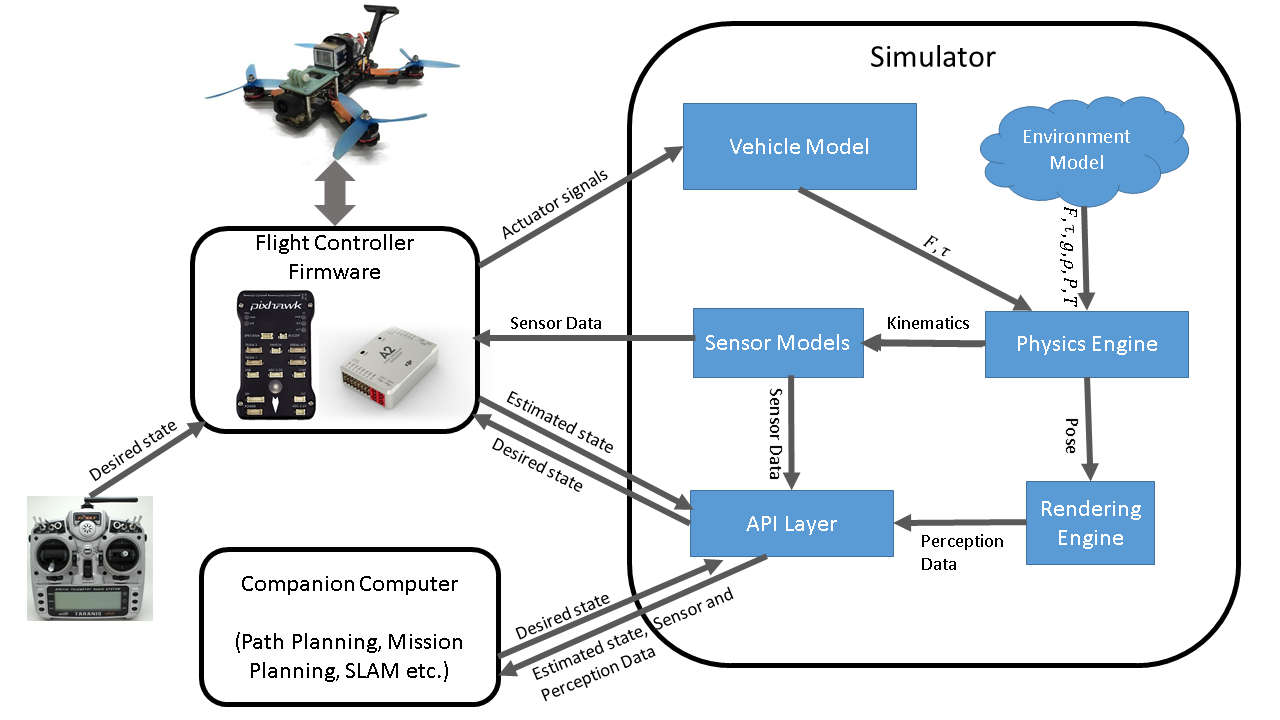
\includegraphics[width=\textwidth,keepaspectratio]{img/airsim-overview.png}
  \caption{High-level overview of how different components interact in the AirSim simulator.}
  \source{Adapted from \citetitle{airsim-paper} \cite{airsim-paper}.}
  \label{fig:airsim-overview}
\end{figure}
\todo[inline]{Final polish: export all boards again from Miro without watermarks}

A high-level overview of the simulator architecture and the way different components interact with each other can be seen in figure~\ref{fig:airsim-overview}. 
The API layer present in the Figure inside the simulator environment refers to AirSim's own airlib library, which exposes with high-level functionality to send control commands to the flight controller directly.
However, in order to share the same control code when simulating flight and in real flight without and not depend on the simulator system, the control commands are sent using the official MavSDK API instead, which allows communication of estimated state, desired state and sensor data directly between the flight controller firmware and the companion computer.

In order to run software-in-the-loop simulation, the PX4 firmware needs to be built from the source code on the Linux platform where it is going to run.
The build system then sets up all the necessary ports for the Mavlink communication and starts a local instance of the NuttX operating system that runs on the actual flight board.
\begin{figure}
  \centering
  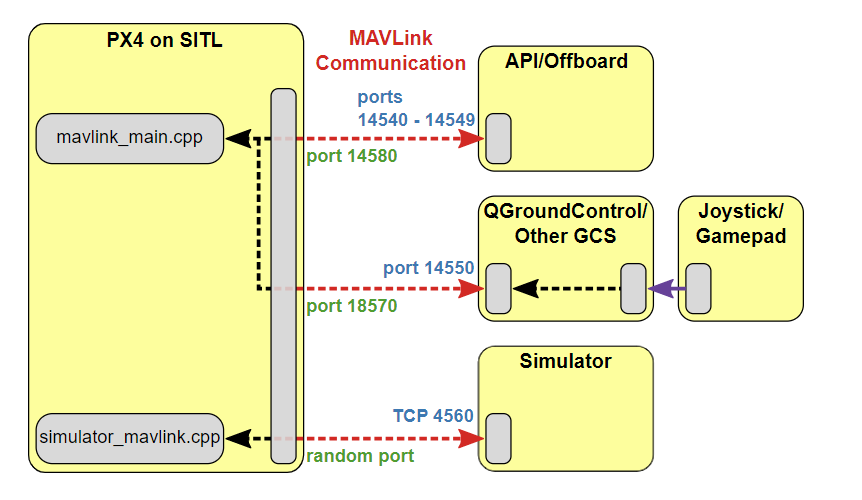
\includegraphics[width=\textwidth,keepaspectratio]{img/px4-ports.png}
  \caption{Network diagram between the different components that interconnect during software-in-the-loop simulation.}
  \source{Adapted from \citetitle{px4-guide} \cite{px4-guide}.}
  \label{fig:px4-ports}
\end{figure}
Figure~\ref{fig:px4-ports} shows how the different parts of the system communicate with each other inside a SITL simulation.
PX4 uses commonly established UDP ports for MAVLink communication with ground control stations (e.g. QGroundControl), offboard APIs (e.g. MAVSDK, MAVROS) and simulator APIs (e.g. AirSim, Gazebo).
External developer application like Dronecontrol use an offboard API, in this case MAVSDK, and therefore listen to PX4's remote UDP port 14540.
All ports in the range 14540-14549 can be used to connect offboard API, for example in the case of controlling multiple vehicles at the same time.
PX4's remote UDP Port 14550 is used for communication with ground control stations, which are expected to listen for connections on this port (QGroundControl listens to this port by default).
PX4 uses a simulation-specific module to connect to the simulator's local TCP port 4560. 
Simulators then exchange information with PX4 using the Simulator MAVLink API shown in Figure~\ref{fig:simulator-msgs}. 
PX4 on SITL and the simulator can run on either the same computer or different computers on the same network.

Since the purpose of using AirSim as a simulator is to run it on a Windows computer and the PX4 software-in-the-loop stack runs on Linux, it is necessary to run a virtualized Linux OS in parallel on the Windows computer and setup a local network so that the simulator and the flight controller firmware can communicate with each other.
The PX4 development team officially supports running the SITL flight stack in Windows through the Windows Subsystem for Linux (WSL2)\footnote{\url{https://docs.microsoft.com/en-us/windows/wsl/about}}, which allows users to install and run their Ubuntu Development Environment on Windows as if it was running it on a Linux computer.
The Windows Subsystem for Linux lets developers run a GNU/Linux environment (including most command-line tools, utilities, and applications) directly on Windows, unmodified, without the overhead of a traditional virtual machine or dualboot setup.
The full steps needed for to configure the system are detailed in Section~\ref{sec:test2}.

\begin{figure}
  \centering
  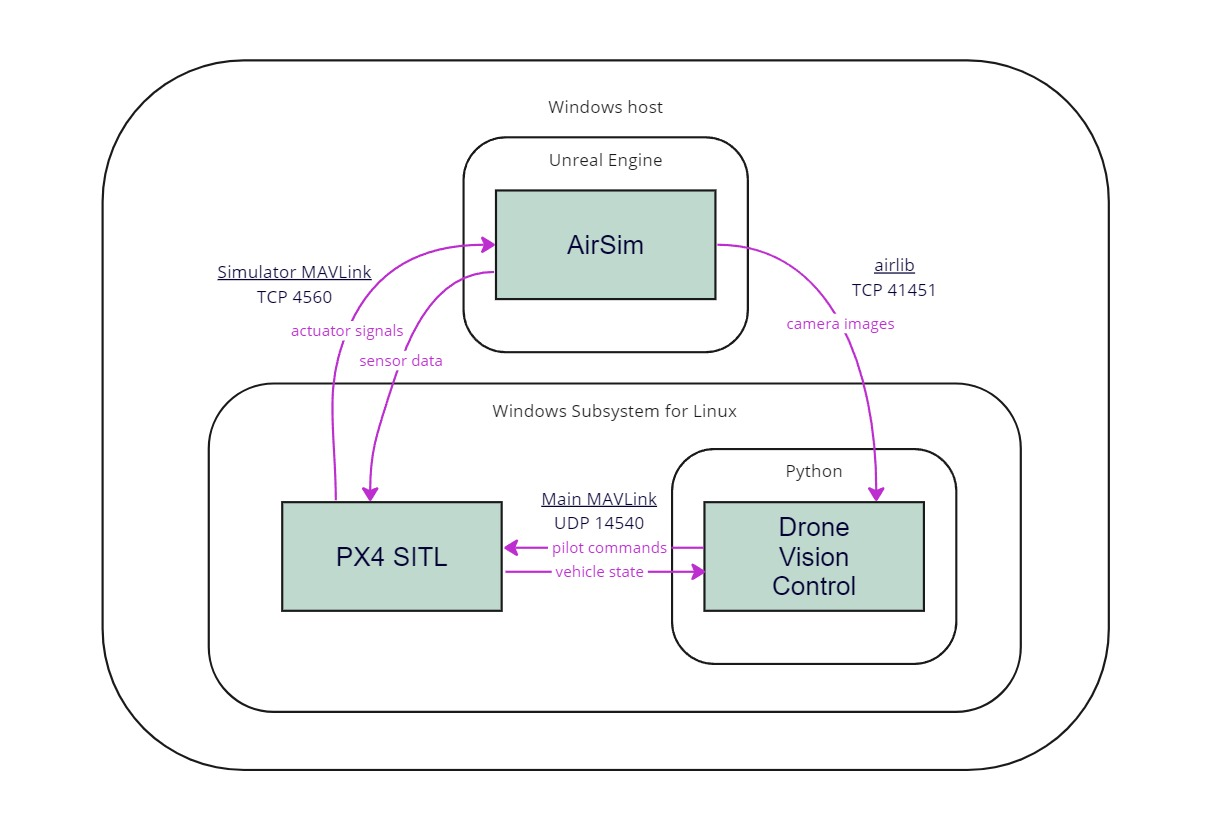
\includegraphics[width=\textwidth,keepaspectratio]{img/sitl-connections.jpg}
  \caption{Connection diagram of how the three systems interact with each other during SITL simulation.}\label{fig:sitl-connections}
\end{figure}
The whole set of connections established in the software-in-the-loop simulation is shown in Figure~\ref{fig:sitl-connections} at the transport layer level. The two systems that run inside the virtualized Linux system through WSL (the simulated flight stack and the dronecontrol program) connect through the localhost network on the UDP port defined by PX4 for Offboard APIs and each of them connects in turn to the AirSim simulator through the virtual Local Area Network established by the Windows Subsystem for Linux to the host Windows computer.
The PX4 flight stack on SITL mode connects to the simulator using the TCP port 4560, as defined by PX4 on Figure~\ref{fig:px4-ports}, and dronecontrol connects through the AirSim library which uses by default a TCP connection on port 41451.

In the case of hardware-in-the-loop simulation, the main difference with SITL is that the flight stack firmware runs on a physical flight board using a special configuration.
In HITL all motors/actuators are blocked, but internal software is fully operational.
This configuration adds an additional separated operating system and to make this mode of testing simpler, since the WSL environment is no longer needed to run the flight stack, it is possible to move the execution of the Python module to Windows.
This eliminates the need to add further configuration to allow the external flight controller to communicate with the internal WSL network, which is by default only accessible by its Windows host computer.
Moreover, now that PX4 runs on a separate piece of hardware, it is necessary to establish two separate physical connections to the Windows computer, so that both the simulator and the Python app can communicate through their own channel to the flight controller, either wired, to the microUSB port or an unused telemetry port on the flight controller, or wireless through a telemetry radio.

\begin{figure}
  \centering
  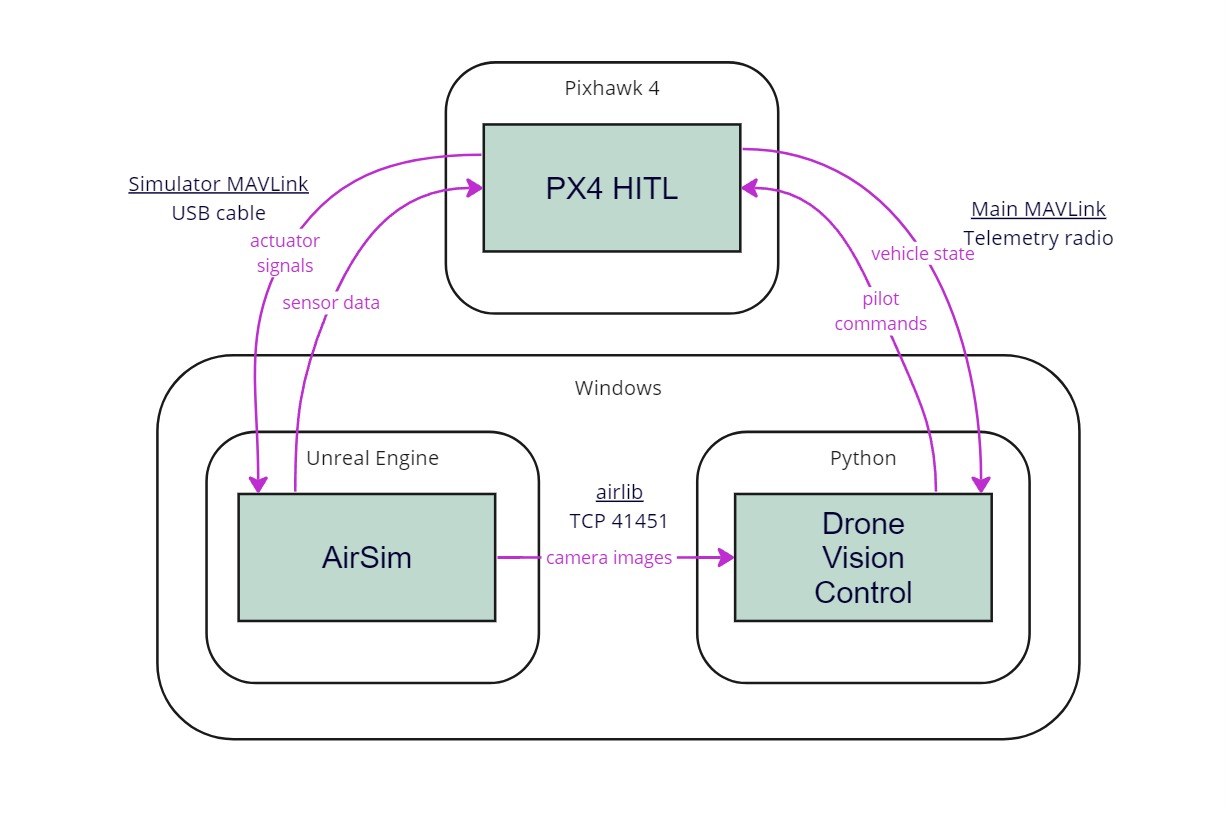
\includegraphics[width=\textwidth,keepaspectratio]{img/hitl-connections.jpg}
  \caption{Connection diagram of how the three systems interact with each other during HITL simulation.}\label{fig:hitl-connections}
\end{figure}

Figure~\ref{fig:hitl-connections} shows the chosen connections to execute tests in HITL mode.
The Windows machine runs both AirSim and the Python interpreter, which communicate through the \texttt{localhost} network using TCP.
The board running PX4 connects to the simulator through a USB to microUSB cable, which is setup to work with a baudrate of 115200, and to the developed program through a telemetry radio running at a baudrate of 57600, both attached to USB ports on the Windows computer accessible through their COM address.

\subsubsection{AirSim testing environment}

Unreal Engine is a complex computer graphics generation program.
It works by creating environments where components like 3D models, cameras, and lighting can be added.
AirSim is a plugin made for this engine by Microsoft, and although it also has a release for the other main game engine in the market, Unity, it is experimental and limited in features.
The documentation contains all the necessary steps to get Unreal Engine and AirSim running on a Windows, Linux, or macOS operating system. 
However, it works best on Windows \cite{build-airsim}.
The source code for the AirSim project includes a built-in Unreal environment that can be used to run tests and contains several 3D shapes like block and spheres, as well as a default quadcopter to act as the control vehicle.
It is also possible to create custom Unreal environments and run AirSim inside them by adding the built plugin to the project and a custom vehicle.

The environment used in this project for testing the Dronecontrol application is derived from the built-in AirSim environment.
It contains the default quadcopter vehicle, which includes several virtual cameras in order to be able to retrieve images from the vehicle's point of view in the simulated world, and a few of the preset blocks with a green color to give a better contrast to the camera.
The main addition to the environment is the 3D model of a human figure, to be used for testing the pose detection and tracking mechanisms of the computer vision solution.
The model is part of a free asset library of human models made by Renderpeople \cite{render-people} obtained in the Unreal Marketplace.
An image of the testing environment can be seen in figure \ref{fig:unreal-env}.


\begin{figure}
  \centering
  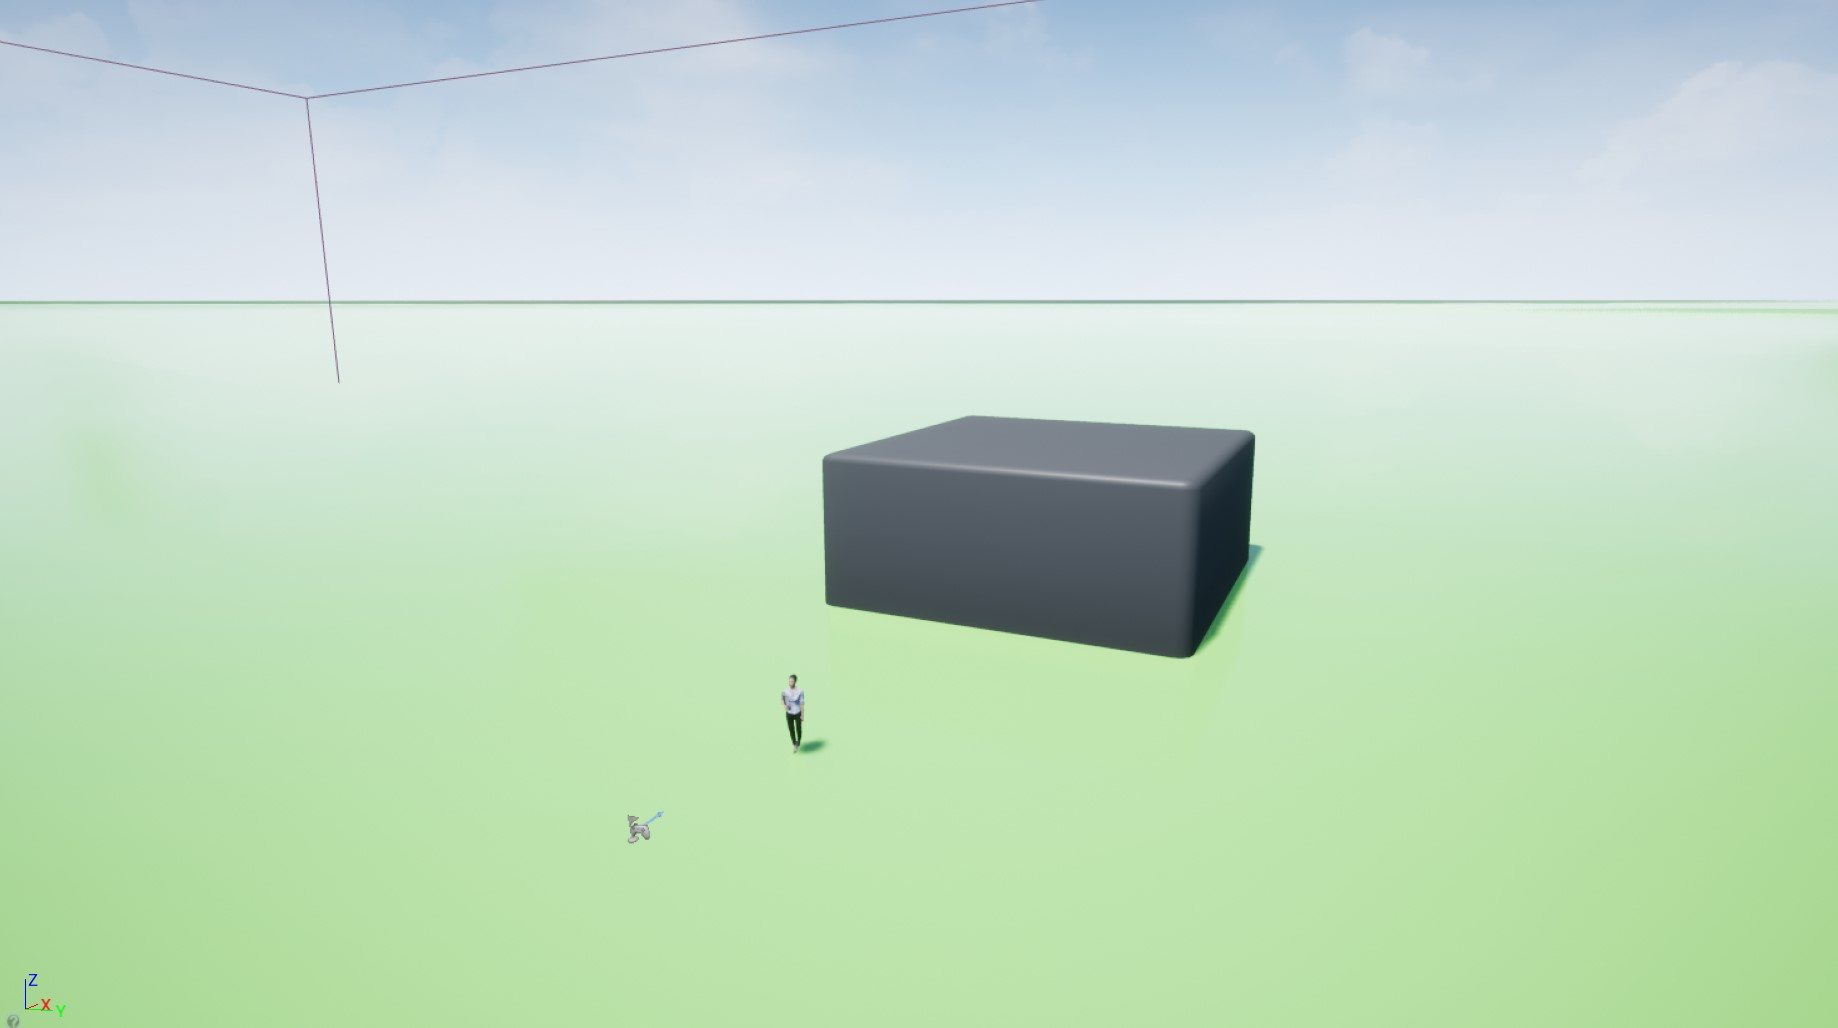
\includegraphics[width=\textwidth,keepaspectratio]{img/unreal-env.jpg}
  \caption{Screenshot from the Unreal Engine environment used for testing the computer vision solutions.}
  \label{fig:unreal-env}
\end{figure}


AirSim is compatible both with SITL and HITL simulation.
However, it is necessary to set it up to work with an external PX4 flight controller instead of AirSim's own internal \texttt{SimpleFlight}.
Appendix \ref{app:airsim-config} shows all the required settings for configuring these modes in AirSim.
To run the simulator in Windows and the flight controller in WSL, the IP of the Windows host in the \texttt{vEthernet (WSL)} network needs to be provided in the AirSim settings.
This process is detailed further in the AirSim documentation \cite{airsim-doc-wsl}.
In brief, first the Unreal project with AirSim has to be set into play mode and then the PX4 SITL flight controller built and run to attach to an already running simulator.
Inside the project in WSL, the flight controller can be run for AirSim by using the provided shortcut script \footnote{\url{https://github.com/l-gonz/tfg-giaa-dronecontrol/blob/main/simulator.sh}}:
\begin{minted}{bash}
sh simulator.sh --airsim
\end{minted}
Once both the simulator and the flight controller are connected, an RC controller or QGroundControl can be used to control the vehicle, and other offboard applications like Dronecontrol can be attached to send any desired MAVLink commands.

\section{System architecture}
\label{sec:sysarch}

\subsection{Top level}

\begin{figure}
  \centering
  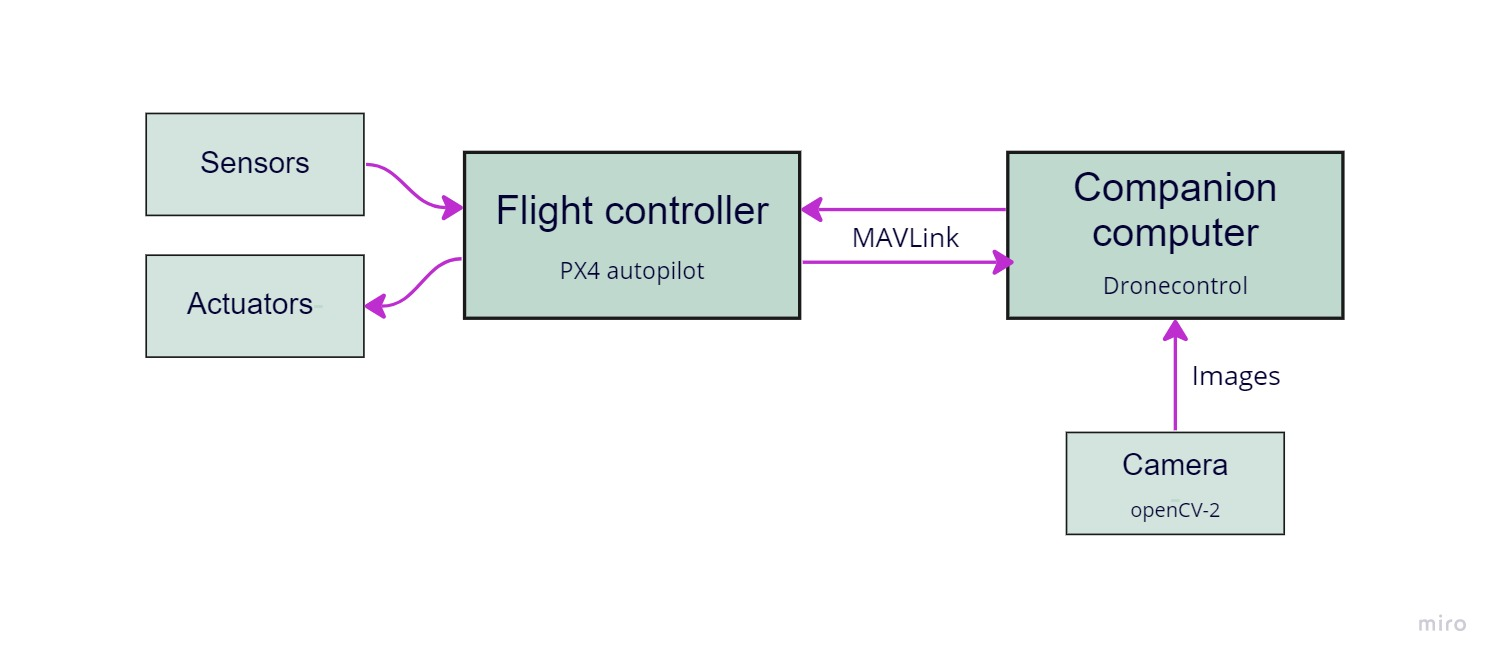
\includegraphics[width=0.9\textwidth,keepaspectratio]{img/sys-arch-diagram.jpg}
  \caption{Top level diagram of the hardware/software interactions}
  \label{fig:toplevel}
\end{figure}

The purpose of the Dronecontrol application is to be able to direct the movement of a \gls{uav} through the analysis of the images taken by a camera.
Since the processing power needed to work with the images recorded is superior to that offered by the autopilot flight controller it becomes necessary the use of an additional companion computer that will control the camera and employ machine learning to extract useful features from the images, as well as transform those features into movement directives for the vehicle.

A top level diagram of the individual parts that comprise the system is shown in Figure~\ref{fig:toplevel}. The main elements are the flight controller, that will run the PX4 autopilot \ref{subsec:px4}, the companion computer, that will run the developed application, and the camera, which provides the images.
The flight controller interfaces directly with the companion computer using the \gls{mavlink} protocol described in Section~\ref{subsec:mavlink}, either through a wireless radio link or a cabled serial connection between the two.
The camera is connected to the companion computer through a cable into an USB port on the computer.
Typically, the type of connection between the flight controller and the computer depends on the desired setup for the system so in the case where the camera, and therefore the companion computer, flies onboard the vehicle it is most convenient to use a direct wire connection between the two, as it provides a faster and more stable link. 
This onboard configuration is further detailed in Section~\ref{subsec:offboard}.
On the other hand, in the case where the companion computer will be acting more like a ground station on an offboard configuration it becomes strictly necessary to communicate with the flight controller through a wireless connection. For this purpose, a pair of telemetry radios provided with the Development Kit of the Holybro X500 (\ref{subsec:pixhawk}) are used. The complete setup requiered for this configuration is described in Section~\ref{subsec:onboard}.

In this project, the flight controller is driven by the PX4 software (\ref{subsec:px4}) and the hardware employed is optimized for this flight stack.
PX4 uses sensors to determine the vehicle state, which is needed for stabilization and to enable autonomous control.
It minimally requires a gyroscope, accelerometer, magnetometer (compass) and barometer.
A GPS or other positioning system is needed to enable all automatic flight modes, and some assisted ones.
PX4 uses outputs to control motor speed, flight surfaces like ailerons and flaps, camera triggers, parachutes, grippers, and many other types of payloads.
Many PX4 drones use brushless motors that are driven by the flight controller via an Electronic Speed Controller (ESC).
The ESC converts a signal from the flight controller to an appropriate level of power delivered to the motor.
PX4 drones are mostly commonly powered from Lithium-Polymer (LiPo) batteries.
The battery is typically connected to the system using a Power Module or Power Management Board, 
which provide separate power for the flight controller and to the ESCs for the motors.
A Radio Control (RC) system is used to manually control the vehicle.
It consists of a remote control unit that uses a transmitter to communicate stick/control positions with a receiver based on the vehicle.
Some RC systems can additionally receive telemetry information back from the autopilot.
Telemetry Radios can provide a wireless MAVLink connection between a ground control station and a vehicle running PX4.
This makes it possible to tune parameters while a vehicle is in flight, inspect telemetry in real-time, change a mission on the fly, etc.

On an actual UAV, the PX4 software runs on a dedicated piece of hardware like the Pixhawk 4 flight controller described in Section~\ref{subsec:pixhawk} that includes all the minimal required sensors for flight as well as interfaces to connect additional actuators and I/O systems (RC, telemetry radio, etc).
However, it is also possible to simulate this hardware on a standard Linux system by building the PX4 source code on a computer with this operating system.
This process is described in the development environment section (\ref{sec:devenv}).

The Dronecontrol application that runs on the companion computer has been developed using the Python programming language \footnote{\url{https://www.python.org/}}.
It offers good advantages for a project of this characteristics because of its high-level,
easy-to-use syntax, that usually results in a smaller code base than other comparable languages for small projects, its versatility and support for object-oriented programming. 
Most importantly, Python is widely used and its official package manager \texttt{pip} greatly simplifies the use of external libraries and which gathers in its package index \footnote{\url{https://pypi.org/}} thousands of standard utilities,
including many machine learning and image processing projects and all the required libraries for interacting with PX4 through the MAVLink protocol (MavSDK).
As it is an interpreted language, it can run easily in any system with Python installed without the need to compile separate binaries for different operating systems.

The next sections explore deeper into the differences between the two configurations mentioned before: offboard computer (or ground station) and onboard computer.

\subsection{Offboard computer configuration}
\label{subsec:offboard}

The offboard configuration allows the flight controller to communicate and receive orders from a companion computer that is not physically connected to its hardware but that can instead stay on ground while the vehicle flies.
This has the advantage that it permits a simpler configuration, without having to be concerned with low-level hardware interactions between the two systems or powering of the companion computer while in flight, as well as allowing the use of a more powerful computer for image processing.
However, it also requires that the camera stays connected to computer on the ground so it cannot use images from the perspective of the drone in flight which limits the real-world applications of the system.
Other configurations involving a direct connection from a camera to the flight controller and the transmission of its images wirelessly to the companion computer through mavlink for processing can be feasible with the current technology but fall out of the scope of this project.

The wireless link is established in this instance through a pair of telemetry radios that connect to a telemetry port on the flight controller and to a USB port in the companion computer, respectively.
Since the Pixhawk 4 is configured by default to used its \texttt{TELEM1} port for this purpose, no additional configuration is needed when using that port.
In the companion computer, applications like the QGRoundControl \footnote{\url{http://qgroundcontrol.com/}} ground station software which is part of the Dronecode Project are able to detect automatically a telemetry radio inserted into any of the USB ports of the host computer.
Additionally, other applications using the MavSDK (\ref{subsec:mavlink}) library can establish connection specifying the baudrate and the USB serial port address, usually something similar to \texttt{/dev/ttyUSB0} on Linux and \texttt{COM1} on Windows.

The radio used for the physical tests in this project is the Holybro SiK Telemetry Radio \footnote{\url{http://www.holybro.com/product/transceiver-telemetry-radio-v3/}}.
It is a small, light and inexpensive open source radio platform that typically allows ranges of better than 300m “out of the box” (the range can be extended to several kilometres with the use of a patch antenna on the ground).
The radios are offered either as 915Mhz (Europe) or 433Mhz (US) so they can be used in different regions and comply with the regulations for frequency, hopping channels and power levels.
They offer 2-way full-duplex communication through an adaptive TDM UART interface and their antenna allows for an adjustable 100-mW-maximum output power and -117 dBm receive sensitivity.
The link is established by default with a baudrate of 57600 (max bits per second on a serial channel) and it can provide air data rates of up to 250 kbps.

\todo[inline]{Take pictures: Images of the radios with computer, flight controller}

\subsection{Onboard computer configuration}
\label{subsec:onboard}

The second way of configuring the interaction between the flight controller and the companion computer consists of integrating both together on board the \gls{uav}.
In this case, the connection is done through a direct cable between the serial port in the flight controller and a USB port in the companion computer.
The camera will then be connected via cable as well to the companion computer and oriented in the vehicle in a way that allows for the best possible perspective during flight.
This configuration makes it possible to develop new control solutions based on images taken directly from the vehicle and that reflect the trajectory that it follows.
Therefore, it becomes possible to adjust the control loop based on previous reactions of the vehicle to commands and maintain a feedback loop for a more stable guidance.

Since the computer running the visual processing algorithm now has to fly on board the vehicle, it becomes specially important to make a good choice when selecting hardware.
To be able to take into the air, the computer has to be light enough that its weight can be lifted by the propellers while maintaining an adequate battery autonomy, but also powerful enough that the processor can handle the computer vision algorithms required to extract the necessary features from the images taken from the onboard camera that are to be feed to the control loop.

\begin{figure}
  \centering
  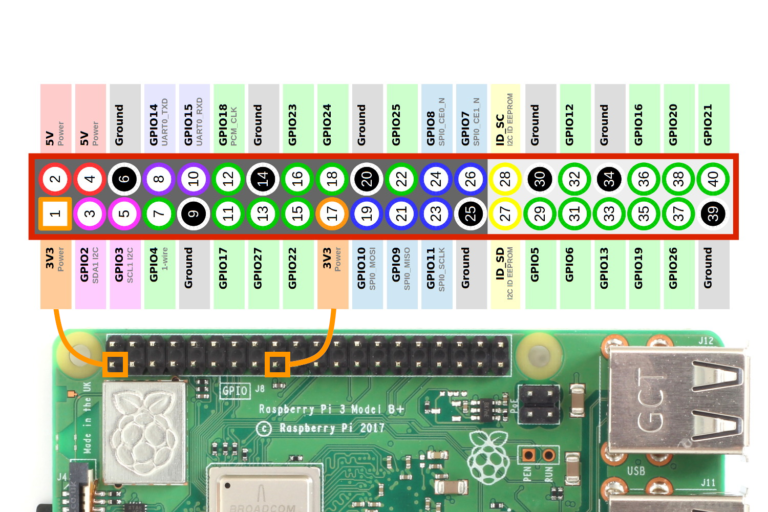
\includegraphics[width=0.8\textwidth,keepaspectratio]{img/rpi4-pinout.png}
  \caption{The Raspberry Pi 4 microcomputer, with its 40-pin GPIO header marked in red, and its pinout.}
  \source{Adapted from \citetitle{rpi4-pinout} \cite{rpi4-pinout}}
  \label{fig:rpi4-pinout}
\end{figure}

The Raspberry Pi 4 model chosen for this project and shown in Figure~\ref{fig:rpi4-pinout} is one of the most popular small computers available in the market at the time, and it is widely use in all kinds of robotics projects both for education and hobbyists.
One of the most important advantages of using such a platform is the easy access to a great amount of manuals, guides and other support available online.
In addition, the Raspberry's officially supported operating system, called Raspberry Pi OS, is a Debian-based version of Unix optimized for its ARM microcontroller, simplifying the process of moving from an Ubuntu test environment into real flight experiments.
Since this computer is designed to be easy to integrate with hardware projects it includes a 40-pin GPIO header (marked in red in Figure~\ref{fig:rpi4-pinout}) that can be programmed for connecting to any number of external devices.


The Raspberry Pi is powered by a 5V input that can be provided either from its USB-C port or through one of two pins in the header dedicated to this (marked as "5v Power" on figure \ref{fig:rpi4-pinout}.
In the case of the particular vehicle build used in this project, the power management board supplying the energy (the Holybro PM07 \footnote{\url{http://www.holybro.com/product/pixhawk-4-power-module-pm07/}}) also provides 5V to the flight controller, as well as powering the ESCs to the motors.
It counts with two power outputs: one of them connected to the flight controller's \texttt{POWER1} port and another one that remains unused.
A first attempt at supplying current to the Raspberry Pi was tested initially with a direct connection between the second, free output on the power module and the powering pins on the GPIO header with a custom connector.
However, the power supply ended up being too unstable for the Pi board, resulting in frequent dips in the supplied current that would affect the processing capabilities of the companion computer.
The solution was to add an additional, secondary battery to the build that provides power through an USB cable.
This configuration allows the Raspberry to receive power by its default way, through the regulated USB-C port.
The disadvantage is that it add one more piece of equipment of substantial weight that needs to be secured to the vehicle's frame and carried into the air while in flight.


In regards to the camera that will fly onboard the vehicle, there are many possibilities to chose from.
The most important characteristics that should be looked for are a small weight and simple plug-and-play interaction with the onboard computer.
The camera used for the tests carried out and detailed in section \ref{chap:validation} is a Logitech C920 1080p webcam \footnote{\url{https://www.logitech.com/es-es/products/webcams/c920-pro-hd-webcam.960-001055.html}}.
Since the frame of the Holybro X500 is not prepared by default to include an onboard camera,
a custom support has been designed and 3D-printed from PLA plastic to be able to hang the camera from the central rods on the underside of the vehicle frame and ensure that it is attached securely during flight.
The 3D model of the custom support can be seen in figure \ref{fig:camera-holder-3d} and the print-ready file can be found in the project repository in GitHub \footnote{\url{https://github.com/l-gonz/tfg-giaa-dronecontrol/blob/main/data/camera-holder.stl}}.
\todo{Final check: link works}

\begin{figure}
  \centering
  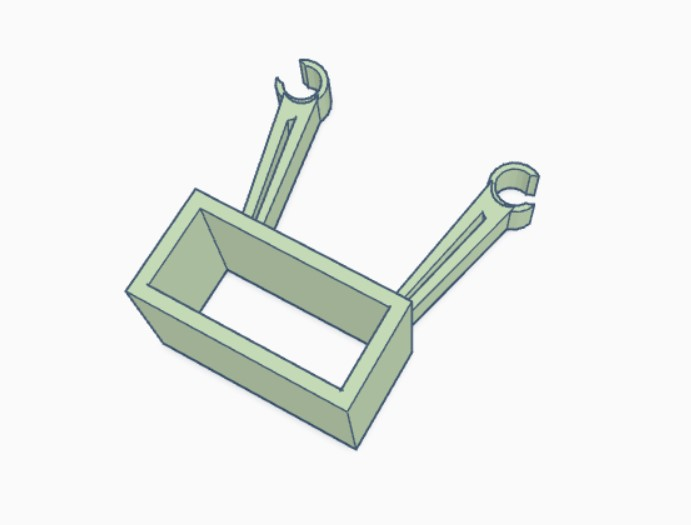
\includegraphics[width=0.6\textwidth, keepaspectratio]{img/cam-holder.jpg}
  \caption{3D model for the camera support designed for the Holybro X500 frame.}
  \label{fig:camera-holder-3d}
\end{figure}


\begin{figure}
  \centering
  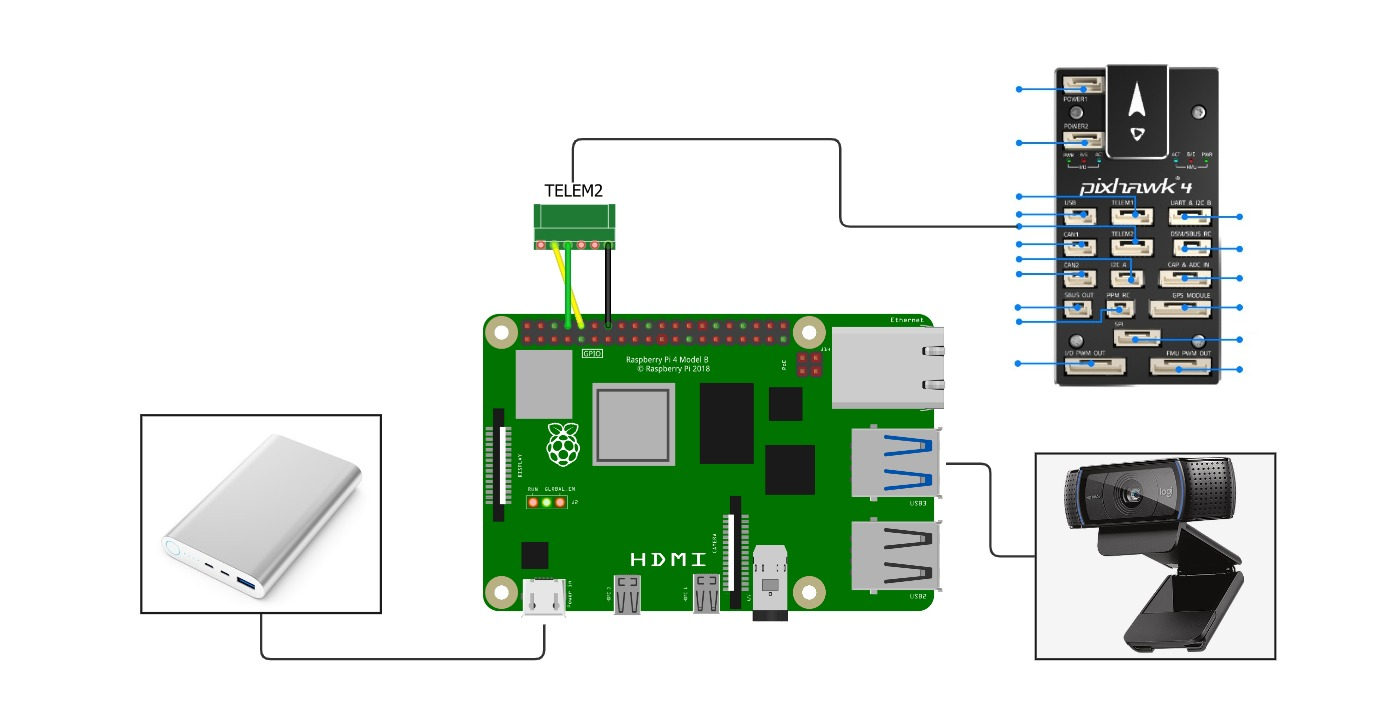
\includegraphics[width=\textwidth,keepaspectratio]{img/wiring-diagram.jpg}
  \caption{A diagram of the wired connections from the Raspberry Pi 4 to the secondary battery and the flight controller (\texttt{TELEM2}).}
  \label{fig:wiring}
\end{figure}


The second wired connection that needs to be established for this configuration is between the flight controller and the companion computer so the Mavlink messages can be exchanged.
As it is desirable to be able to maintain a wireless link to the vehicle even while it is being controlled by the onboard computer, the telemetry radio is kept connected to the \texttt{TELEM1} port of the flight controller and the companion computer is wired to the \texttt{TELEM2} port.
This port is not configured to be used by default so it is necessary to modify the configuration of the Pixhawk board either through QGroundControl or the PX4 console.
The required parameter to change in the board is mainly the \texttt{MAV\_1\_CONFIG}, which configures the serial port on which to run a second instance of MAVLink (primary instance is configured with \texttt{MAV\_0\_CONFIG}), and defaults to 0 (disabled) and should be set to 102 for TELEM 2.
This MAVLink instance is set to Onboard mode by default, which is the appropriate mode for communicating with an offboard computer, instead of the Normal mode running on the primary MAVLink instance through \texttt{TELEM1} to communicate with QGroundControl.
Another parameter to take into account is the \texttt{SER\_TEL2\_BAUD}, which regulates the baud rate of the \texttt{TELEM2} port.
The default rate is 921600, and it needs to be used when establishing connection in the Dronecontrol application through the MAVSDK library.
PX4 provides a complete overview of all the available parameters for the board configuration in their documentation \cite{px4-docs-params}.



The other end of the connector has three female Dupont wires that go into the TX/RX UART pins of the Raspberry Pi,
according to mapping table \ref{tab:wiring-telem} between the 6 pins in the telemetry connection of the Pixhawk board and the corresponding GPIO pins in the Raspberry Pi header \cite{pixhawk-manual} \cite{pixhawk-px4}.
A diagram of all the connections to the companion computer can be seen in figure \ref{fig:wiring}.

\begin{table}[]
\centering
\begin{tabular}{|ll||ll|}
\hline
\multicolumn{2}{|c||}{\textbf{TELEM2}}                                             & \multicolumn{2}{c|}{\textbf{GPIO header}}                                        \\ \hline \hline
\multicolumn{1}{|c|}{\textit{Pin \#}} & \multicolumn{1}{c||}{\textit{Description}} & \multicolumn{1}{c|}{\textit{Description}} & \multicolumn{1}{c|}{\textit{Pin \#}} \\ \hline
\multicolumn{1}{|l|}{1}               & VCC, +5V                                  & \multicolumn{1}{l|}{}                     &                                      \\ \hline
\multicolumn{1}{|l|}{2}               & TX (out), +3.3V                           & \multicolumn{1}{l|}{GPIO15 (RXD0, UART)}  & 10                                   \\ \hline
\multicolumn{1}{|l|}{3}               & RX (in), +3.3V                            & \multicolumn{1}{l|}{GPIO14 (TXD0, UART)}  & 8                                    \\ \hline
\multicolumn{1}{|l|}{4}               & CTS (in), +3.3V                           & \multicolumn{1}{l|}{}                     &                                      \\ \hline
\multicolumn{1}{|l|}{5}               & RTS (in), +3.3V                           & \multicolumn{1}{l|}{}                     &                                      \\ \hline
\multicolumn{1}{|l|}{6}               & GND                                       & \multicolumn{1}{l|}{GND}                  & 6                                    \\ \hline
\end{tabular}
\caption{Mapping between the \texttt{TELEM2} port in the Pixhawk 4 board and the Rapberry Pi's GPIO header.}
\label{tab:wiring-telem}
\end{table}

In comparison with the default baudrate of 57600 on the telemetry radio link established in the previous section the wired serial connection works at a baudrate of 921600, which means that data can be transferred 16 times faster through the link.
%Main limitation is image processing though, so slower processing power from computer means slower responsiveness to movement all together. Any info about update rate from PX4? Does it depend on the link speed or is it constant?
\todo[inline]{Final polish: link to performance section}

The offboard configuration allowed the supervision of the output from the program while the vehicle was flying, since the computer stayed stationary on the ground, however in this configuration it is not possible to have a screen connected directly to the companion computer.
To fix this situation and be able to monitor during flight, as well as being able to give input directly to the program, it is possible to make use of the WiFi receptor of the Raspberry Pi to configure a remote desktop and connect to it through another computer serving as a ground station;
then the output from the camera and the image recognition can be seen in real time.

Figure \ref{fig:onboard-config} shows a summary of all the connections mentioned between the autopilot the companion computer, and their respective peripherals.
\todo[inline]{Write: elaborate on the summary}

\begin{figure}
  \centering
  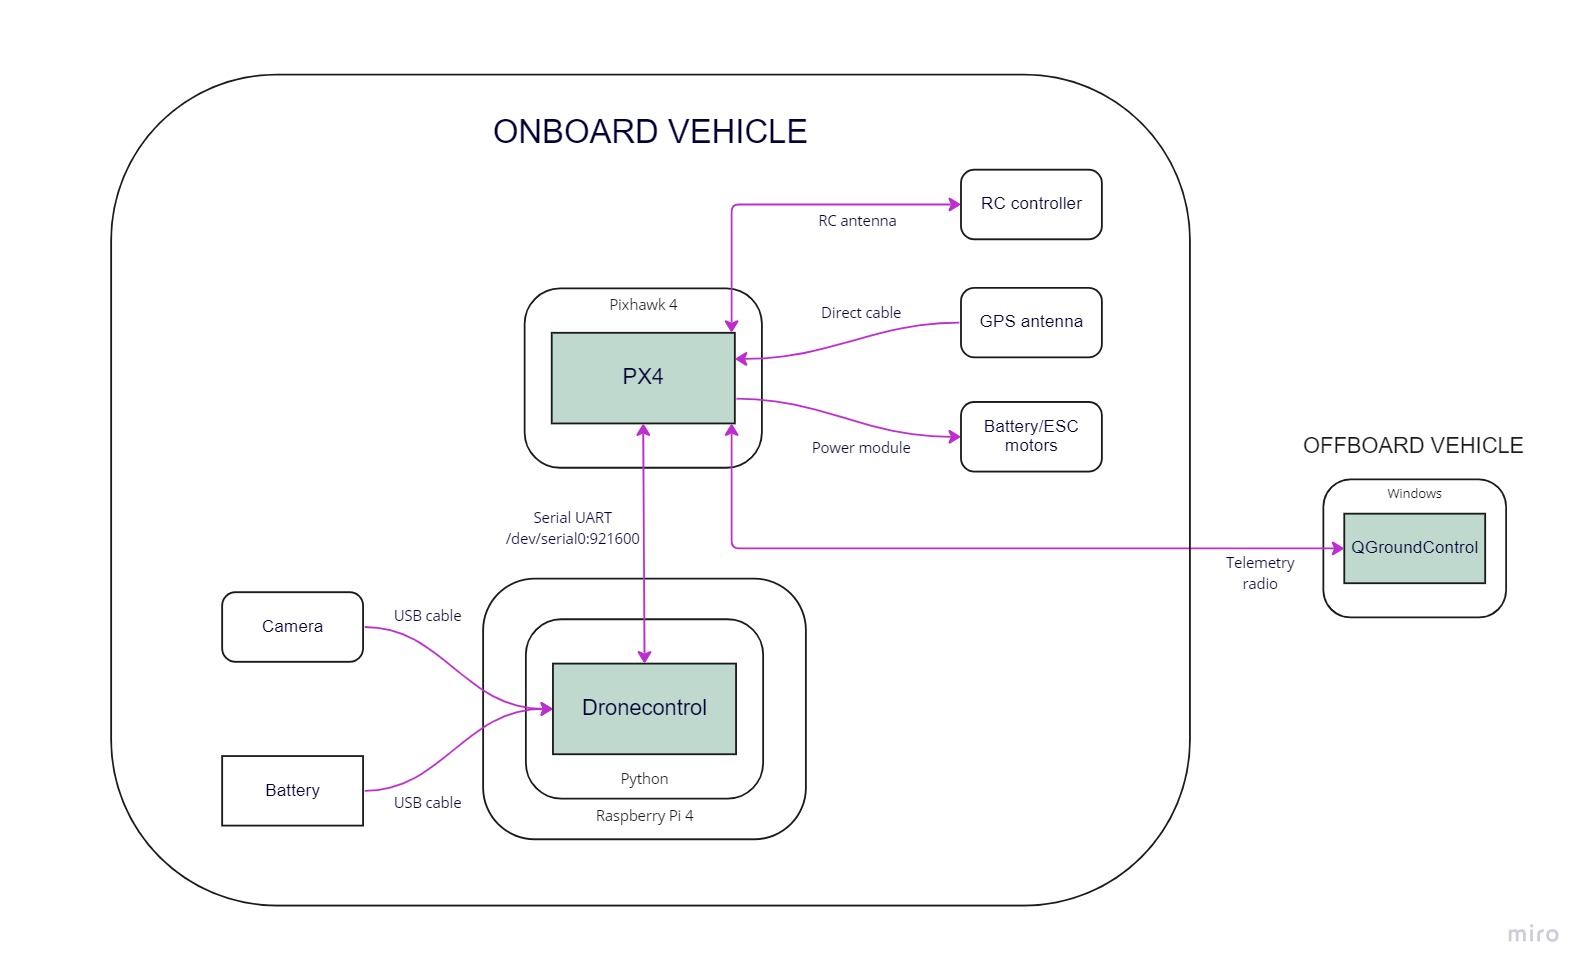
\includegraphics[width=\textwidth,keepaspectratio]{img/onboard-diagram.jpg}
  \caption{Onboard configuration connections}
  \label{fig:onboard-config}
\end{figure}

\section{Software architecture}

\begin{figure}
  \centering
  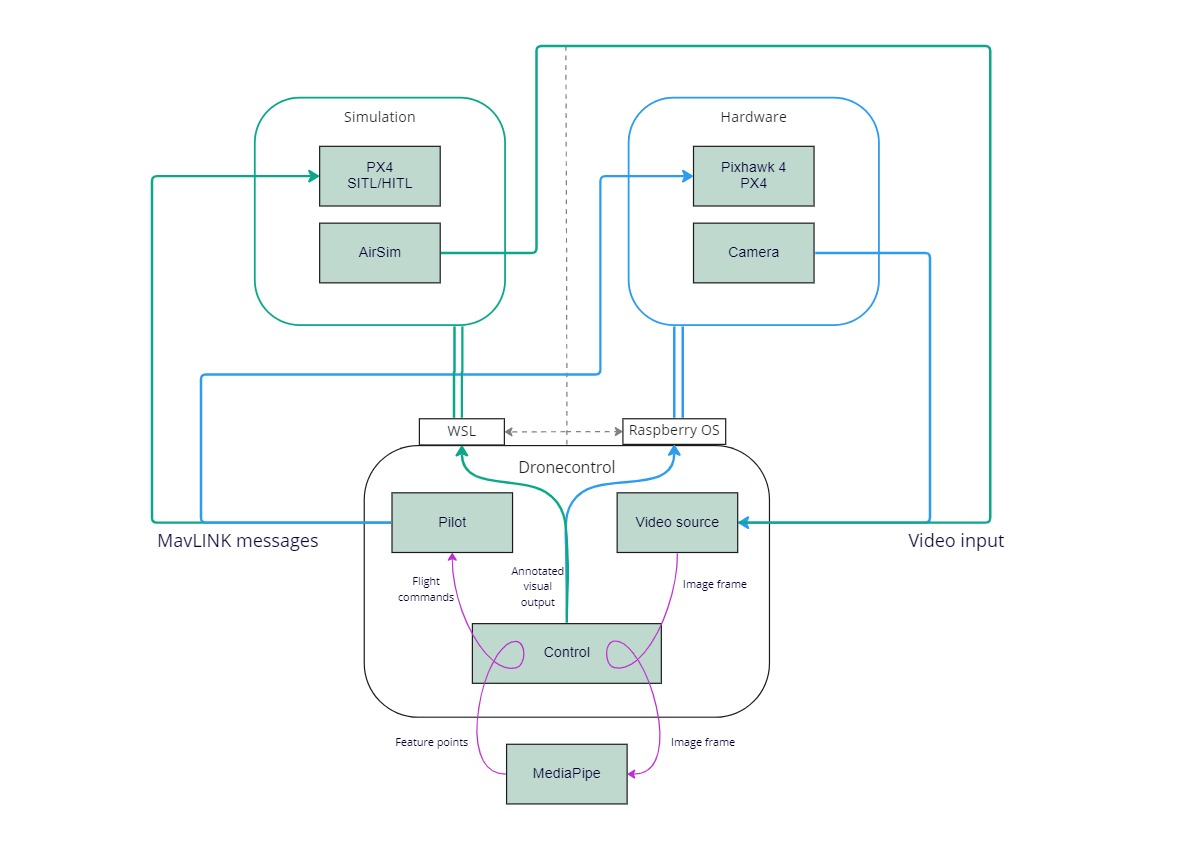
\includegraphics[width=\textwidth, keepaspectratio]{img/software-arch.jpg}
  \caption{Structure of the program}\label{fig:architecture}
\end{figure}

\todo[inline]{Write: Describe the actual new diagram, blue vs green arrows, data flow, ...}

Figure \ref{fig:architecture} shows the main modules the designed the software is composed of and how it interacts with the external libraries.
The application consists of three basic parts: 
the pilot module, in charge of sending instructions to the flight controller and receiving back information on position and state through the \texttt{mavsdk} library, 
a video source module that handles the retrieval of images from different sources and the necessary processing for image analysis, 
and a control module that directs the interaction between the other two to transform the pixel information first into position points through the \texttt{mediapipe} library and then into instructions for the pilot.
The upper part of the diagram in figure \ref{fig:architecture} shows how the program modules receive input and send instructions to the hardware systems whether these are simulated or not.
Other smaller utilities have also been developed to help test how the systems interact with each other and calibrate different parts of the control behaviour.
Appendix \ref{app:cli} contains the user manual with all the application's options.

\subsection{Pilot module}
The purpose of the pilot module is to provide access to the rest of the application to send and receive messages from the PX4 controller through the MavSDK library.
This library provides a simple asynchronous API for managing one or more vehicles, providing programmatic access to vehicle information and telemetry, and control over missions, movement and other operations.
MavSDK utilizes the python standard library \emph{asyncio} to be able to run coroutines in parallel while waiting for the messages provided through the \emph{MAVLink} communication.
Therefore all calls to the library have to be written as async functions that await the result of one or more polls to the flight stack.

\texttt{asyncio} provides support for writing concurrent code using the \texttt{async/await} syntax.
It is used as a foundation for multiple Python asynchronous frameworks that provide high-performance network and web-servers, database connection libraries, distributed task queues, etc; 
and provides a set of high-level APIs to run Python coroutines concurrently and have full control over their execution.
The pilot module integrates \texttt{mavsdk} and \texttt{asyncio} and provides a queue for the control module to send actions to be executed in the vehicle one after another.

Listing~\ref{lst:pilot.connect} shows how to establish a connection to a PX4 vehicle through its physical (serial) or virtual (UDP) address and poll for internal information from the flight controller to decide when the system is ready to receive instructions.
The mavsdk library exposes telemetry and other state information through asynchronous generators, which are defined in python as a convenient way to make asynchronous data producers and accessed with the \mintinline{python}{async for} syntax.


\begin{listing}[h!]
    \caption{Example of how the communication to the flight stack is established through asyncio and the mavsdk library}{}
    \label{lst:pilot.connect}
    \begin{minted}[breaklines, fontsize=\footnotesize, baselinestretch=1]{python}
async def connect(self):
    """Connect to mavsdk server.
       Raises a TimeoutError if it is not possible to establish connection.
    """
    
    if self.serial:
        address = f"serial://{self.serial}"
    else:
        address = f"udp://{self.ip if self.ip else ''}:{self.port}"
    self.log.info("Waiting for drone to connect on address " + address)
    await asyncio.wait_for(self.mav.connect(system_address=address), timeout=self.TIMEOUT)

    async for state in self.mav.core.connection_state():
        if state.is_connected:
            break

    # Wait for drone to have a global position estimate
    async for health in self.mav.telemetry.health():
        if health.is_global_position_ok:
            break
        
    self.log.info("System ready")
    self.is_ready = True
    \end{minted}
\end{listing}

Many of basic operations that can be executed in the flight controller are implemented in the pilot module with error handling and safety checks, like takeoff, landing, return home or manipulating the vehicle flying velocity directly by providing speeds in body coordinates.
These actions can be executed directly or added to a queue that runs in on a loop executing them in the order they are added, waiting until the previous action has finished and the vehicle is in the desired state before starting the next.
The loop that runs this queue can be seen in Listing~\ref{lst:pilot.queue}.
There is a maximum time of 10 seconds that each action can use to run
The loop stops when the asynchronous task it runs on is cancelled with \mintinline{python}{task.cancel()}, which raises a \mintinline{python}{CancelledError} exception in the parallel execution.

\begin{listing}[h!]
    \caption{Loop where the action queue runs on the pilot module. Each action is awaited until it finishes or the timeout time runs out.}{}
    \label{lst:pilot.queue}
    \begin{minted}[breaklines, fontsize=\footnotesize, baselinestretch=1]{python}
async def run_queue(self):
    """
    Run the queue loop.
    
    Queued actions will be awaited one at a time
    until they are finished.
    The loop will sleep if the queue is empty.
    """
    try:
        while True:
            if len(self.actions) > 0:
                action = self.actions.pop(0)
                self.log.info("Execute action: %s", action.func.__name__)
                try:
                    await asyncio.wait_for(action.func(self, **action.args), timeout=10)
                except asyncio.exceptions.TimeoutError:
                    self.log.warning(f"Time out waiting for {action.func.__name__}")
            else:
                await asyncio.sleep(self.WAIT_TIME)
    except asyncio.exceptions.CancelledError:
        self.log.warning("System stop")
    \end{minted}
\end{listing}

\subsection{Video source module}

The objective of the video source module is to provide a collection of classes to retrieve images from different sources,
in a way that they can be exchanged for one another without affecting the rest of the application to facilitate testing and be adaptable running in different environments.
There are three classes of video sources implemented: file, simulator and camera, which inherit from the same \mintinline{python}{VideoSource} base class as shown in Figure~\ref{fig:video-source-inheritance}.

\begin{figure}
  \centering
  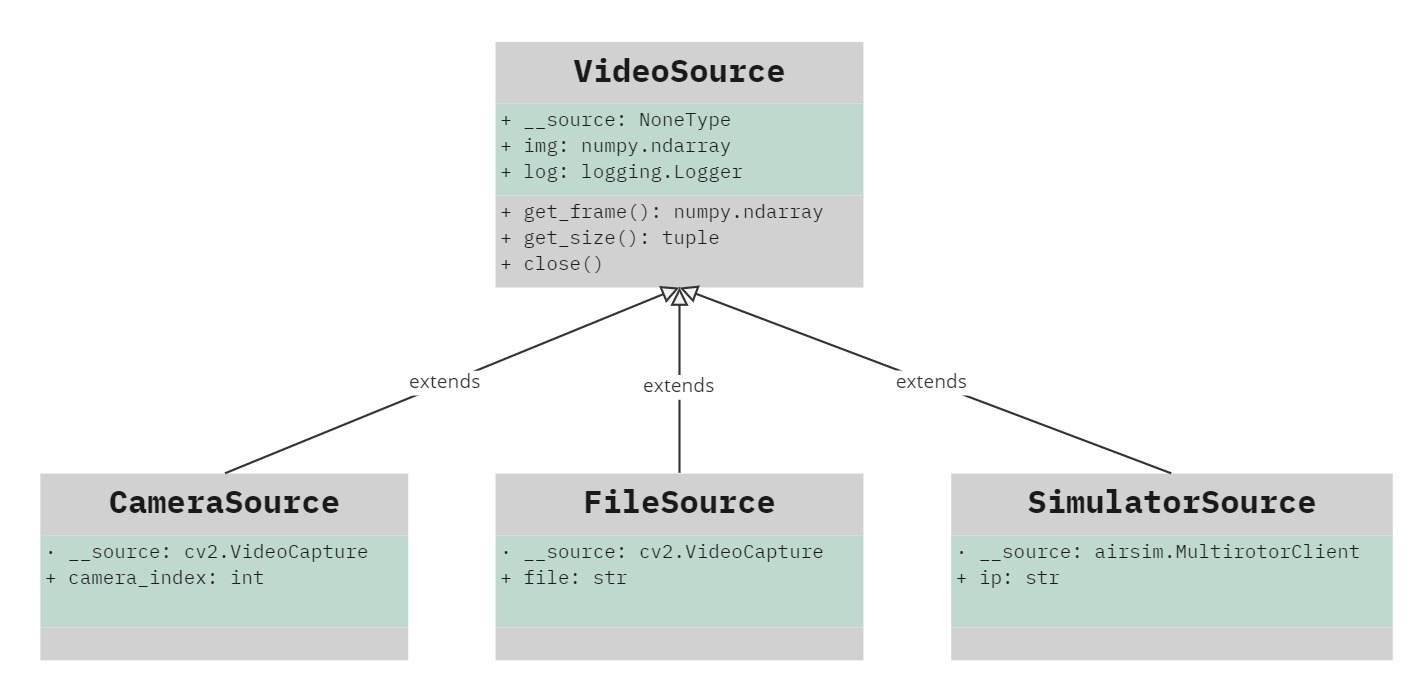
\includegraphics[width=8cm, keepaspectratio]{img/uml-video-source.jpg}
  \caption{Diagram of inheritance on the video source classes available to retrieve image data.}
  \label{fig:video-source-inheritance}
\end{figure}

The \mintinline{python}{FileSource} class is able to open a video file stored in the companion computer and provides images taken frame by frame from it until the video ends.
This allows the program to replay the image detection algorithms on videos previously captured by the camera tool exposed in section~\ref{subsec:test-tools}.
The \mintinline{python}{CameraSource} class can access a physical camera attached to the computer running the application via USB and provide the frames captured in real time.
Both the file and camera sources employ OpenCV's video capture utilities to take care of the file handling and the camera driver management capabilities respectively.

The simulator source uses AirSim's Python library to communicate with the simulator and retrieve images from a simulated camera attached to the 3D model of the vehicle in Unreal Engine.
It connects automatically through localhost, but it can also be provided with an IP to establish connection to the simulator running on a different computer on the local network, for example when the program runs inside WSL and the simulator runs on its host computer.

\subsection{Vision control module}
The control module contains the main logic of the application and is in charge of converting the raw images obtained from the video source into commands for the pilot module.
Two different types of control have been implemented.
The first one is a proof-of-concept control solution, described in section \ref{sec:hands}, that runs in offboard mode (see section \ref{subsec:offboard}) and translates some predefined hand gestures into simple commands for the aerial vehicle, of which the main purpose is to be able to test the interaction between all the components of the system in a more easily controlled environment, since it uses the simpler configuration of situating the computer with the controller outside of the vehicle.
The second control system consists of a follow solution more applicable to real-life scenarios where the control and the camera is onboard the vehicle and the presence of a person is detected in the images obtained from the perspective of the drone in order to be able to give the flight controller velocity commands to follow said person and maintain it centered in its view.

The process followed in both solutions consists roughly of the same two parts.
First the image is sent to the computer vision and machine learning third-party library that extracts the required features from the image in the form of 2D coordinates.
Afterwards a series of calculations depending on the particular solution are applied to these coordinates to decide which commands are sent to the pilot module.
The third-party library used for computer vision in the program is the mediapipe library described in Section~\ref{subsec:mediapipe}, which offers cross-platform, customizable ML solutions for live and streaming media, specifically its hand and pose detection solutions.

To engage the module in direct control of the vehicle's velocity it is necessary to use a special flight mode defined by PX4 for this purpose, called Offboard Mode \footnote{\url{https://docs.px4.io/main/en/flight_modes/offboard.html\#offboard-mode}} (not to be confused with the offboard configuration described in section~\ref{subsec:offboard}).
Offboard mode is primarily used for controlling vehicle movement and attitude, and supports only a very limited set of MAVLink messages. This mode requires position or pose/attitude information to be available to the flight controller, e.g. GPS.
In it, the vehicle obeys a position, velocity or attitude setpoint provided over MAVLink by a MAVLink API (i.e. MAVSDK) running on a companion computer and usually connected via serial cable or wifi.
A stream of setpoint commands must be received by the vehicle at a rate higher than 2Hz prior to engaging the mode and in order to remain in it.
If the message rate falls below 2Hz or the connection is lost the vehicle will stop and, after a timeout, the vehicle will attempt to land or perform some other failsafe action according to the parameters configured.
In order to hold position while in this mode, the vehicle must receive a stream of setpoints for the current position.

Sections~\ref{sec:hands} and \ref{sec:follow} offer a more complete explanation of the control module used by the two different solutions developed.

\subsubsection{Camera-testing tool}
\label{subsec:test-tools}

Several additional utilities have been added to the dronecontrol program to facilitate the development and testing process of the two main control solutions.
The first tool is accessed through the command \mintinline{bash}{dronecontrol tools test-camera} and can be used for testing the connection between the computer and the camera, as well as the performance of the MediaPipe hand and pose machine learning solution on real time images.
It is as well possible to take images and record video from the live camera feed for later analysis and it allows connecting to a physical or simulated flight controller to send basic commands through keyboard input like takeoff and landing.

\todo[inline]{Write: Add control functionality, describe connection options, link to cli in appendix}
\todo[inline]{Polish: Link some code from test-camera tool}





\section{Proof of concept: hand-gesture solution}
\label{sec:hands}
The main purpose of this solution is to test that the flow of the application works as expected, both in simulation and in real flight, and that all the systems are capable of establishing the required connections with each other.
For that reason it is designed to be able to be run in real flight with the minimal setup of a built drone with its default components and any computer with a camera.

\begin{figure}
  \centering
  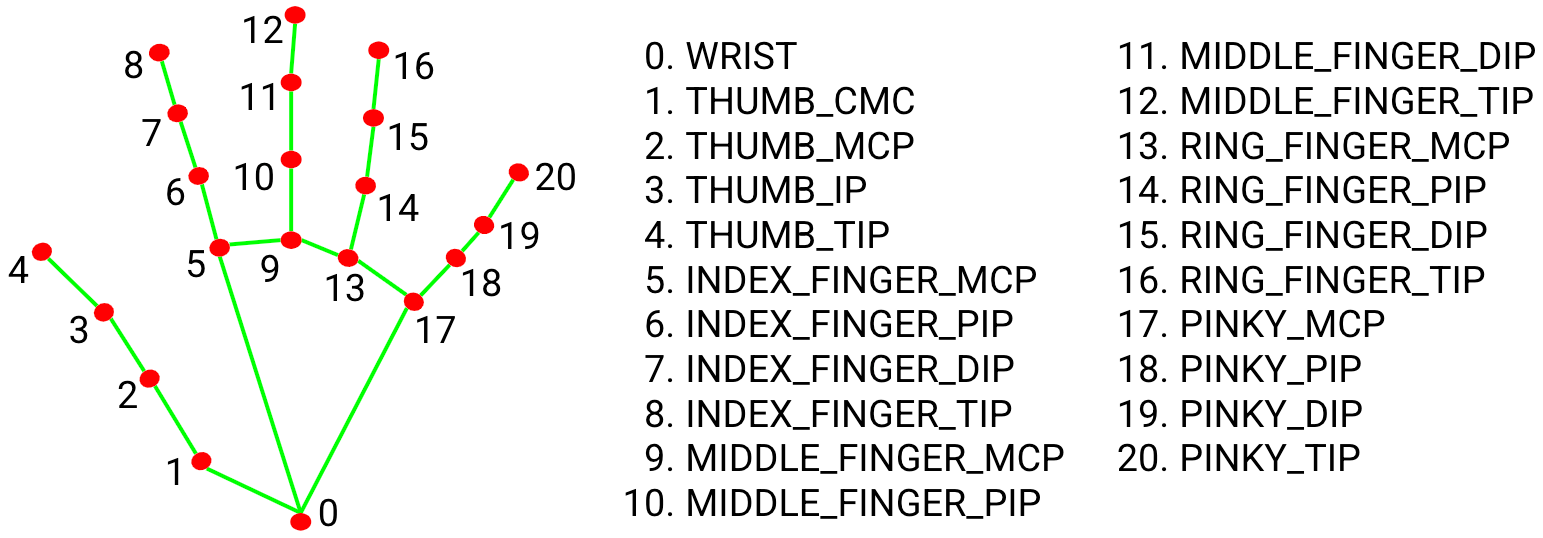
\includegraphics[width=\textwidth, keepaspectratio]{img/hand_landmarks.png}
  \caption{Landmarks extracted from detected hands by the MediaPipe hand solution.}
  \source{Adapted from \citetitle{mp-hands} \cite{mp-hands}.}
  \label{fig:hand-landmarks}
\end{figure}

This control module runs on a loop that continuously polls for a new frame from the chosen video source and feeds it to the hand detection functionality from MediaPipe \cite{mp-hands-paper}.
If a hand is detected in the images, 2D coordinates are extracted according to the map shown in figure~\ref{fig:hand-landmarks}.
These landmarks are then converted into different discrete gestures like open palm, closed fist or an specific finger pointing different directions.
When a new gesture is detected, the command assigned to it is queued to the pilot module and executed as soon as the previous commands end their execution.

The conversion between landmarks and gestures is performed by drawing vectors from the base of each of the fingers to their tips as well as from the base of the hand (wrist feature) to the base of the fingers and using the dot product vector operation to calculate the relative angles between each finger and the base of the hand, as shown in figure~\ref{fig:vector-calcs}.
By comparing the calculated angles to a threshold, it is possible to detect whether each individual finger is extended or folded, as well as the general direction it is pointing towards.
The open hand gesture, for example, can then be defined as all five fingers extended, that is, all five vectors defined by the fingers sharing the same approximate angle with the vector from the base of the hand to that finger.

\begin{figure}
  \centering
  
\includegraphics[width=8cm, keepaspectratio]{img/placeholder.png}
  \caption{Vector calculations}
  \label{fig:vector-calcs}
\end{figure}
\todo[inline]{Draw: hand vectors}

The full list of gestures detected by the program by calculating these angles is as follows:
\begin{itemize}
    \item No hand: happens when no landmarks are able to be extracted from the image. As a safety feature, in this case the vehicle stops whichever previous commands it had in its queue and goes into hold flight mode, where it just hovers in the air maintaining its position.
    \item Open hand: it is detected when all five fingers are extended, as if gesturing stop, and makes the drone land at its current position.
    \item Fist: it is detected when all five fingers are folded and makes the drone arm and takeoff. If the drone is already in the air nothing happens.
    \item Index finger pointing up: it is detected when only the index finger is extended and it is pointing roughly towards the top of the image ($\pm 30$ degrees) and makes the drone go into offboard mode, where it is possible to receive direct velocity commands.
    \item Index finger pointing to the right: same as above but pointing to the right of the image and makes the drone roll towards its right side at a speed of 1 m/s.
    \item Index finger pointing to the left: same as above but the drone rolls towards its left side.
    \item Thumb pointing to the right: it is detected when index finger is extended up (to maintain the drone in offboard control) and the thumb is extended pointing towards the right of the screen. This gesture makes the drone pitch forward at a steady speed of 1 m/s.
    \item Thumb pointing to the left: same as the previous gesture, but the drone pitches backward when the thumb point to the left of the screen.
\end{itemize}

\todo[inline]{Write: add loop code and link to first paragraph}
\todo[inline]{Draw: Include diagram of angles for each pointy gesture ?????}
\todo[inline]{Images: simulators program output image with drawn lines for gestures}
\todo[inline]{Video: hand control in simulator}





\section{Final solution: human following}
\label{sec:follow}

The intention behind the development of a UAV control solution that implements tracking and following of humans is to show how the PX4 open-source development platform and its related projects, MAVLINK and MAVSDK, can be used to design complex real-life applications without the need for expensive state-of-the-art proprietary hardware.
The only requirements of the follow application are a PX4-enabled flight controller installed in an aerial vehicle, a companion computer of appropriate dimensions to be able to be mounted on board the vehicle and any camera that can be connected to the companion computer via USB.
During the program execution, the drone can be controlled via an RC controller, an external ground station application or keyboard input directly to the companion computer through, for example, a secure shell using the SSH protocol.

For safety, the follow mechanism only engages when the flight mode on the vehicle is changed to offboard mode e.g. by activating a configured switch in the RC controller, and stops automatically if the connection to the computer is lost or any of the available failsafes are triggered, like low battery, loss of RC or GPS signal or vehicle attitude exceeding a predefined pitch and roll value for longer than a specified time.
In this mode the vehicle will attempt to find a single person in its field of view and follow their movements by changing its yaw and forward velocity to match horizontal movements and distance changes, respectively.

\begin{figure}
  \centering
  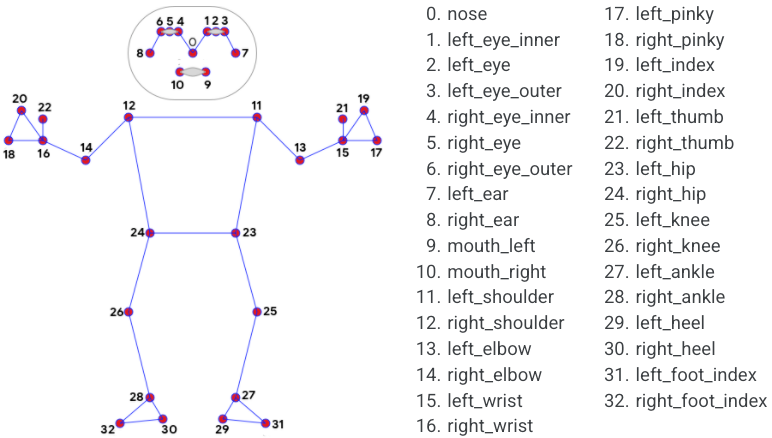
\includegraphics[width=\textwidth, keepaspectratio]{img/pose-landmarks.png}
  \caption{Landmarks extracted from detected human figures by the MediaPipe Pose solution}
  \source{Adapted from \citetitle{mp-pose} \cite{mp-pose}}
  \label{fig:pose-landmarks}
\end{figure}

During the program execution and while the offboard mode and the follow mechanism is engaged, the system continuously retrieves images from the offboard camera that are fed into the MediaPipe Pose \cite{mp-pose-paper} computer vision library to extract pose landmarks from it in the form of 2D coordinates.
Figure~\ref{fig:pose-landmarks} shows the available extracted features and their correspondence to the human body.
These coordinates are used to draw a bounding rectangle around the detected person, as well as for validating that the received landmarks match the general pose of a person standing up.
To prevent unwanted movements, the vehicle will always stop and hover every time it becomes impossible to detect a person in the image received or its features do not match the expected geometry.
\todo[inline]{Images: valid and invalid person detection from simulator camera output}
After a valid bounding box has been defined around the target person, its position in respect to the field of view of the camera is sent to a control mechanism composed of two independent PID controllers. The theory behind these controllers is explained in section~\ref{subsec:pid-tools}).

The first of the PID controllers is in charge of controlling the yaw velocity of the vehicle to respond to horizontal movements in the x direction of the image. 
\todo[inline]{Draw: coordinate system figure}
It takes as input the x coordinate of the center point of the bounding box and its target is the middle point of the screen.
This controller therefore will output velocity commands aimed to maintain the bounding box centered horizontally in its field of view.

The second PID controller controls the forward velocity of the vehicle to respond to distance changes of the person getting closer or further away from the drone.
It takes as input the height of the calculated bounding box as a percentage of the total height of the field of view and works to keep it within a value that matches the desired distance to maintain between the person and the vehicle by moving forwards when the height is too low and backwards when it is to high.
The exact percentage of the image height that is covered by a person at a given distance depends on the camera used and needs to be obtained empirically for each separate video source.

\todo[inline]{Add some controller and follow code to show and explain}
\todo[inline]{Images: simulator and output, link video of run}



\subsubsection{PID tools}

Two additional utilities have been developed for tuning and measuring the performance of the PID controllers.
\todo[inline]{Write: PID tools, how they work and code}
\todo[inline]{PID library, Formula and coefficients}

%%%%%%%%%%%%%%%%%%%%%%%%%%%%%%%%%%%%%%%%%
\begin{equation}
    u(t)= K_p e(t) + K_i \int{e(t)dt} + K_d \frac{de(t)}{dt}
%    \caption{Formula for the output from a PID controller}
    \label{eq:pid}
\end{equation}
%% Where: $u(t)=$ PID control variable
        % $K_p=$ proportional gain
        % $K_i=$ integral gain
        % $K_d=$ derivative gain
        % $e(t)=$ error value
        % $de=$ change in error value
        % $dt=$ change in time
%%%%%%%%%%%%%%%%%%%%%%%%%%%%%%%%%%%%%%%%%

The process of tuning the PID controllers is described in section~\ref{sec:test-1-pid}


\subsection{Safety mode}
\label{subsec:safety}

\todo[inline]{Write: safety mechanisms, speed limits on pids, loss of signal, loss of vision, ...}
\todo{}
\todo{}


\cleardoublepage

% EXPERIMENTOS Y VALIDACIÓN %
\chapter{Experiments and validation}
\label{chap:validation}

\section{PID tuning and controller validation}

% Process of tuning the PIDs
% Graphs from test-controller
% Analysis of error

\section{Testing the software-in-the-loop simulation}

% Setup:    build from source code on WSL
% Test:     - Jmavsim simulator
%           - Hand solution: (on Python Windows?????)
%               - Mediapipe
%               - Pilot module
%               - Video input
% Results:  images from jmavsim, dronecontrol output, px4 console

\section{Testing the AirSim simulator}

% Setup:    installing AirSim, AirSim config explanation
% Test:     - AirSim simulator
%           - Follow solution:
%               - Pose detection
%               - Images from simulator
%               - Control from PIDs
%               - Failsafes
% Results:  images from airsim, dronecontrol output, px4 console

\section{Testing the hardware-in-the-loop simulation}

% Setup:    build drone, HITL configuration
% Test:     - AirSim + follow on Windows + Pixhawk
%           - QGroundControl (without program running)
%           - PX4 to computer connection
%           - RC on AirSim
% Results:  images of wiring computer-Pixhawk

\section{Testing the Raspberry Pi as the companion computer}

% Setup:    Raspberry Pi installation, RPi-Pixhawk connection
% Test:     - AirSim + follow on RPi + Pixhawk
%           - Serial connection
% Results:  wiring, performance metrics

\section{Testing the onboard camera}

% Setup:    installing AirSim, AirSim config explanation
% Test:     - AirSim + hand-solution on RPi + Pixhawk + onboard camera
%           - Camera holder
% Results:  holder 3d, drone close-up, camera feed

\section{Testing a fully-built drone}

% Setup:    build drone, configuration, calibration
% Test:     - RC, GPS, Pixhawk power supply, RPi power supply
%           - Arm, takeoff commands
% Results:  wiring, drone pictures, QGroundControl calibration screens

\section{First flight tests}

% Setup:    flight plan
% Test:     - takeoff with QGC, fly with RC
%           - tools/test_camera + record video
% Results:  video of flying

\section{Hand solution in real flight scenarios}

% Setup:    ...
% Test:     - Hand solution on windows through telemetry radio
%           - Free movement with offboard api
% Results:  video of flying, output from program

\section{Follow solution in real flight scenarios}

% Setup:    ...
% Test:     - Follow solution on RPi
%           - Controller response to real input
% Results:  video of flying, output from program
            

\cleardoublepage

% CONCLUSIONES %
\chapter{Conclusions}
\label{chap:conclusion}

\todo[inline]{Write: short recap with conclusions}


\section{Evaluation of objectives}
\label{sec:consecucion-objetivos}

% Esta sección es la sección espejo de las dos primeras del capítulo de objetivos, donde se planteaba el objetivo general y se elaboraban los específicos.
% Es aquí donde hay que debatir qué se ha conseguido y qué no. 
% Cuando algo no se ha conseguido, se ha de justificar, en términos de qué problemas se han encontrado y qué medidas se han tomado para mitigar esos problemas.
\todo[inline]{Write: Go through objectives in introduction and debate what's been achieved}


\section{Lessons learned}
\label{sec:lessons-learned}

\todo[inline]{Write: Subsection 1 - cosas aprendidas del grado aplicadas al proyecto }
\todo[inline]{Write: Subsection 2 - cosas aprendidas del tfg en general }


\section{Future work}
\label{sec:fut-work}

\todo[inline]{Write: future work}

% Ningún proyecto ni software se termina, así que aquí vienen ideas y funcionalidades que estaría bien tener implementadas en el futuro.

% Es un apartado que sirve para dar ideas de cara a futuros TFGs/TFMs.

% GLOSARIO(S) %
% \printglossary[type=\acronymtype]
% \printglossary

% APÉNDICE(S) %
\cleardoublepage
\appendix
\chapter{Installation manuals}

This appendix 
\url{https://github.com/l-gonz/tfg-giaa-dronecontrol}

\section{SITL: Development environment}
\label{app:install-dev-env}

This section describes the process of installing all the necessary applications to set up a development environment to run PX4's SITL simulation in a system similar to the one described in section \ref{sec:devenv}.
The instructions assume a computer running Windows 10/11 as the operating system and Windows Subsystem for Linux installed.
PX4 details the installation steps of their source code for several platforms in their documentation \cite{install-px4}, where Ubuntu is the recommended platform.
To make it easier, the dronecontrol repository contains a small shell script that aggregates all the steps and installs all the dependencies with the folder structure that the project expects.
This includes installing and setting up PX4 and QGroundControl and creating a virtual environment for the project, installing the Python packages and the dronecontrol application.

To run the script, simply clone the repository, navigate to the project folder and execute:
\begin{minted}[breaklines, fontsize=\footnotesize, baselinestretch=1]{bash}
./install.sh
\end{minted}

To test the installation of PX4, execute the following line (requires a graphic interface for WSL):
\begin{minted}[breaklines, fontsize=\footnotesize, baselinestretch=1]{bash}
./simulator.sh --gazebo
\end{minted}

To test the installation of dronecontrol, execute:
\begin{minted}[breaklines, fontsize=\footnotesize, baselinestretch=1]{bash}
dronecontrol tools test-camera -s -c
\end{minted}
Camera input is not supported from within WSL, but it should be possible to control the simulated drone with the keyboard.

The next step is to install dronecontrol in the Windows machine to be able to access an integrated or USB camera.
It requires having Python already installed.
First, clone the project repository, navigate to the folder and set up the virtual environment:
\begin{minted}[breaklines, fontsize=\footnotesize, baselinestretch=1]{bash}
pip install virtualenv
virtualenv venv
venv\Scripts\activate
\end{minted}

Then install dronecontrol:
\begin{minted}[breaklines, fontsize=\footnotesize, baselinestretch=1]{bash}
pip install -r requirements.txt
pip install -e .
\end{minted}

Additionally, to make the simulated PX4 application broadcast to the Windows machine on port 14550, it is necessary to edit the file \texttt{px4-rc.mavlink} located in \texttt{Firmware/PX4-Autopilot/etc/init.d-posix} on the project folder in WSL.
To the mavlink start command for the ground control link on line 14, append -p to enable broadcasting:
\begin{minted}[breaklines, fontsize=\footnotesize, baselinestretch=1]{bash}
mavlink start -x -u $udp_gcs_port_local -r 4000000 -f
\end{minted}

To test the installation, with the PX4 simulator still running in WSL, execute:
\begin{minted}[breaklines, fontsize=\footnotesize, baselinestretch=1]{bash}
dronecontrol tools test-camera -s -c
\end{minted}
It should now be possible to both control the drone with the keyboard and obtain images from a camera attached to the computer, as well as run the hand control solution in the simulator.

\subsection{Installation of AirSim}

To run the PX4 software-in-the-loop simulator in AirSim and test the follow solution,
first, install Unreal Engine at version 4.27 at least from the Epic Games Launcher\footnote{\url{https://www.unrealengine.com/download}} and open the environment found in the \texttt{data} folder of the repository.
To use AirSim with a different Unreal environment, follow the guide in the AirSim documentation\footnote{\url{https://microsoft.github.io/AirSim/unreal_custenv/}}
After starting play mode in Unreal for the first time, a \texttt{settings.json} file will appear in an AirSim folder in the user's Documents folder.
The contents of this file need to be replaced with the configuration file found in section \ref{app:airsim-config} to be able to interact with PX4 running inside WSL, selecting the correct value for \texttt{"UseSerial"} and exchanging the \texttt{"LocalHostIp"} in the file for the IP of the Windows machine in the virtual WSL network.
This IP can be obtained by typing \texttt{ipconfig} in the Windows command prompt and looking for the IPv4 address under "Ethernet Adapter vEthernet (WSL)".

After the settings have been set, restart play mode in Unreal; the output log should show a message saying "Waiting for TCP connection on port 4560, local IP <Windows-IP>".
It is now possible to build and start PX4 by executing in WSL:
\begin{minted}[breaklines, fontsize=\footnotesize, baselinestretch=1]{bash}
./simulator.sh --airsim
\end{minted}

If the IP has been set correctly in the AirSim settings, 
PX4 and the simulator will find each other correctly and connect.
The test-camera tool can be run either from Linux within WSL or from Windows by executing:
\begin{minted}[breaklines, fontsize=\footnotesize, baselinestretch=1]{bash}
dronecontrol tools test-camera -s -w
\end{minted}

The follow control solution can be run from Linux with:
\begin{minted}[breaklines, fontsize=\footnotesize, baselinestretch=1]{bash}
dronecontrol follow --sim 172.19.112.1
\end{minted}
and from Windows with:
\begin{minted}[breaklines, fontsize=\footnotesize, baselinestretch=1]{bash}
dronecontrol follow --sim -p 14550
\end{minted}

\section{HITL: Installation on a Raspberry Pi 4}
\label{app:install-dronecontrol-rpi}

Install dronecontrol
        
Set up XRDP to connect from windows PC
\url{https://linuxize.com/post/how-to-install-xrdp-on-raspberry-pi/}

Set up UART serial connection in RPi: 
\url{https://discuss.px4.io/t/talking-to-a-px4-fmu-with-a-rpi-via-serial-nousb/14119?page=2}


\section{AirSim configuration file}
\label{app:airsim-config}
\begin{minted}[breaklines, fontsize=\footnotesize, baselinestretch=1]{json}
{
    "SettingsVersion": 1.2,
    "SimMode": "Multirotor",
    "ClockType": "SteppableClock",
    "Vehicles": {
        "PX4": {
            "VehicleType": "PX4Multirotor",
            "LockStep": true,
            "UseSerial": "<true: HITL, false: SITL>"
            "UseTcp": true,
            "TcpPort": 4560,
            "ControlIp": "remote",
            "ControlPortLocal": 14550,
            "ControlPortRemote": 14570,
            "LocalHostIp": "<Windows-IP>",
            "Sensors":{
                "Barometer":{
                    "SensorType": 1,
                    "Enabled": true
                }
            },
            "Parameters": {
                "NAV_RCL_ACT": 1,
                "NAV_DLL_ACT": 0,
                "COM_RCL_EXCEPT": 7,
                "LPE_LAT": 47.641468,
                "LPE_LON": -122.140165
            }
        }
    },
    "CameraDefaults": {
        "CaptureSettings": [
            {
                "ImageType": 0,
                "Width": 640,
                "Height": 400
            }
        ]
    }
}
\end{minted}

\chapter{Command-line interface of the application}
\label{app:cli}

\begin{minted}[breaklines, fontsize=\footnotesize, baselinestretch=1]{bash}
Usage: dronecontrol tools test-camera [OPTIONS]

Options:
  -s, --sim TEXT        attach to a simulator through UDP, optionally provide
                        the IP the simulator listens at
  -r, --hardware TEXT   attach to a hardware drone through serial, optionally
                        provide the address of the device that connects to PX4
  -w, --wsl             expects the program to run on a Linux WSL OS
  -c, --camera          use a physical camera as source
  -h, --hand-detection  use hand detection for image processing
  -p, --pose-detection  use pose detection for image processing
  -f, --file TEXT       file name to use as video source
  --help                Show this message and exit.


Usage: dronecontrol tools tune [OPTIONS]

Options:
  --yaw / --forward     test the controller yaw or forward movement
  --manual              manual tuning
  -t, --time INTEGER    sample time for each of the values to test
  -p, --kp-values TEXT  values to test for Kp parameter
  -i, --ki-values TEXT  values to test for Ki parameter
  -d, --kd-values TEXT  values to test for Kd parameter
  -h, --help            Show this message and exit.


Usage: dronecontrol tools test-controller [OPTIONS]

Options:
  --yaw / --forward  test the controller yaw or forward movement
  -f, --file TEXT    file name to use as data source
  -h, --help         Show this message and exit.


Usage: dronecontrol hand [OPTIONS]

Options:
  -i, --ip TEXT       pilot IP address, ignored if serial is provided
  -p, --port INTEGER  port for UDP connections
  -s, --serial TEXT   connect to drone system through serial, default device
                      is /dev/ttyUSB0
  -f, --file PATH     file to use as source instead of the camera
  -l, --log           log important info and save video
  -h, --help          Show this message and exit.


Usage: dronecontrol follow [OPTIONS]

Options:
  --ip TEXT          pilot IP address, ignored if serial is provided
  -p, --port TEXT    pilot UDP port, ignored if serial is provided, default is
                     14540
  --sim TEXT         run with AirSim as flight engine, optionally provide ip
                     the sim listens to
  -l, --log          log important info and save video
  -s, --serial TEXT  use serial to connect to PX4 (HITL), optionally provide
                     the address of the serial port
  -h, --help         Show this message and exit.
\end{minted}

% \chapter{PX4 parameters}
%%% Maybe %%%
% All parameters changed from their default values
% Connect Pixhawk to QGC, then check config for changed values


% BIBLIOGRAFIA %
\cleardoublepage
% https://www.overleaf.com/learn/latex/Bibliography_management_with_biblatex
\raggedright\printbibliography[heading=bibintoc,title={References}]

\end{document}
